\documentclass[12pt]{article}

\usepackage[margin=1in]{geometry}
\usepackage{setspace}
\usepackage{fontspec}
\IfFileExists{microtype.sty}{\usepackage{microtype}}{}
\usepackage{amsmath, amssymb, amsthm, mathtools}
\usepackage{booktabs}
\usepackage{graphicx}
\usepackage{subcaption}
\usepackage{multirow}
\usepackage{array}
\usepackage{float}
\usepackage{enumitem}
\usepackage[font=small,labelfont=bf]{caption}
\usepackage{tikz}
\usetikzlibrary{positioning}
\usepackage{hyperref}
\usepackage[nameinlink,noabbrev]{cleveref}
\usepackage[round,authoryear]{natbib}

\defaultfontfeatures{Ligatures=TeX,Scale=MatchLowercase}
\IfFontExistsTF{TeX Gyre Termes}{
  \setmainfont{TeX Gyre Termes}
}{
  \setmainfont{Times New Roman}
}
\IfFontExistsTF{TeX Gyre Heros}{
  \setsansfont{TeX Gyre Heros}
}{
  \setsansfont{Helvetica}
}

\setstretch{1.65}
\allowdisplaybreaks
\setlength{\emergencystretch}{3em}

\numberwithin{equation}{section}

\newtheorem{theorem}{Theorem}[section]
\newtheorem{proposition}[theorem]{Proposition}
\newtheorem{lemma}[theorem]{Lemma}
\newtheorem{assumption}[theorem]{Assumption}
\newtheorem{definition}[theorem]{Definition}
\newtheorem{remark}[theorem]{Remark}
\newtheorem{corollary}[theorem]{Corollary}

\newcommand{\mainfigwidth}{0.96\textwidth}
\newcommand{\mediumfigwidth}{0.88\textwidth}
\newcommand{\smallfigwidth}{0.74\textwidth}

\renewenvironment{abstract}{
  \begin{center}
  \bfseries Abstract
  \end{center}
  \vspace{-0.7em}
  \begingroup
  \small
  \setstretch{1.18}
  \noindent
}{
  \par
  \endgroup
}

\makeatletter
\renewcommand{\maketitle}{%
  \begin{center}
    {\Large \@title \par}
    \vspace{0.7em}
    {\normalsize \@author \par}
    \vspace{0.35em}
    {\small \@date \par}
  \end{center}
  \vspace{0.7em}
}
\makeatother

\hypersetup{
  colorlinks = true,
  linkcolor = blue,
  citecolor = blue,
  urlcolor = blue,
  pdfauthor = {Cheikh A. M. Ndiaye},
  pdftitle = {No Country for Honest Men: Balanced Theft, Endogenous Patronage, and the Emergence of Enforcement}
}

\title{No Country for Honest Men:\\
Balanced Theft, Endogenous Patronage, and the Emergence of Enforcement}
\author{Cheikh A. M. Ndiaye\\
Université Laval\\
\href{mailto:candi12@ulaval.ca}{candi12@ulaval.ca}}
\date{March 2026}

\begin{document}
\maketitle

\begin{abstract}
A unit transfer raiding game can sustain equality when each household leaves home, each unoccupied house is targeted once, and concurrent raiders would otherwise divide the same loot. \emph{The Black Sheep} turns on the breakdown of that reciprocal order, and this paper formalizes the sequence. In the benchmark stage game, a balanced theft cycle is a weak Nash equilibrium. In the repeated benchmark with stationary Markov behavior, one permanently honest household stays home, blocks the raid directed at it, and creates a first-night windfall for the adjacent successor in the old cycle. If leaving home exposes current wealth, that windfall moves the successor above the threshold at which personal raiding ceases to be optimal, so the original cycle cannot persist as a stationary continuation. A proportional loot extension then studies the later transition. Rich households hire thieves when delegated predation yields surplus over the worker outside option and contracting cost, and they later replace thieves with guards when concentrated wealth and prey depletion raise the value of protection above the value of one more round of predation. Simulations implement the same payoff comparisons and record the timing of class differentiation, patronage, selective protection, inequality, and welfare loss once theft, contracting, guarding, and punishment consume resources. A local honest rupture can therefore dissolve a reciprocally corrupt order without producing an impartial institutional exit.
\end{abstract}

\noindent \textbf{Keywords:} repeated games, corruption equilibria, patronage, endogenous enforcement, inequality
\par\noindent \textbf{JEL classification:} C73, D74, K42, O17

\section{Introduction}

In \emph{The Black Sheep}, Calvino begins from a society in which theft is universal and equality survives only because every household is both predator and prey. Losses and gains offset one another exactly, so the social order remains predatory without becoming stratified. The story changes when one man stays at home. The raid directed at his house fails, the house he would have robbed remains untouched, and a local disturbance in the transfer network appears at once. The later movement toward hierarchy, delegation, and policing follows from that break \citep{calvino_1993}. The opening order can be written as a unit transfer raiding game in which each household chooses in every period whether to stay home or which other house to raid, occupied houses are safe in the benchmark, and concurrent raiders divide a rival loot whose expected share falls with congestion. Under a balanced theft cycle every household leaves home, every unoccupied house is targeted once, and wealth remains level because each household has one incoming loss and one outgoing gain. Universal predation is then compatible with equality through exact accounting, and that opening order survives as a weak Nash equilibrium of the stage game.

In the repeated version, the horizon is infinite, behavior is restricted to stationary Markov strategies, and one household is permanently honest and therefore remains at home in every period. If the remaining households follow the old cycle on the first perturbed date, the predecessor who targets the honest house returns empty handed, the successor escapes the raid that would otherwise have hit him, and the resulting wealth change is local but exact. Once leaving home also exposes current wealth, the successor's windfall can move him above the cutoff at which personal raiding ceases to be privately attractive, so the original balanced cycle no longer survives as a stationary continuation. A richer environment becomes necessary at that point, because exact unit transfers cannot carry hierarchy very far once wealth begins to diverge. The extension therefore preserves the same population, the same public wealth state, and the same logic of explicit target choice while replacing unit loot with proportional loot and enlarging the occupational menu. Rich households compare personal raiding, staying home, hiring thieves, and later hiring guards; poor households compare freelance theft, paid predation, protection work, and withdrawal. Patronage requires delegated predation to reach targets more effectively than freelancers can and poor workers to face outside options weak enough to leave a surplus after wages and contracting cost. Guarding appears later, once concentrated wealth and prey depletion alter the ranking of control technologies. Hierarchy, delegation, and selective protection then emerge as successive environments, each tied to its own payoff comparison and transition condition.

Several literatures meet naturally at that point. Corruption equilibria remain privately coherent because each participant takes as given an order that depends on the participation of others \citep{andvig_moene_1990,bardhan_1997,shleifer_vishny_1993,tirole_1996}. Local perturbations then matter through the same logic that convention and equilibrium selection models use to study movement across sustained orders \citep{young_1993}. Appropriation and defense enter once predation and protection compete for resources under insecure claims \citep{skaperdas_1992,grossman_kim_1995,hirshleifer_1995}. Hierarchy enters once the rich use vertical organization to redirect predatory labor \citep{olsen_torsvik_1998}. Organized enforcement enters once protection stabilizes an unequal order created during the transition itself \citep{olson_1993,north_wallis_weingast_2009,besley_persson_2009,acemoglu_ticchi_vindigni_2011}. The graph of the balanced benchmark also recalls a directed exchange cycle, which is why \citet{shapley_scarf_1974} remains useful as a limited structural reference. The connection stops at the graph. Transfers here are coercive, occupancy changes the opportunity set of others, and rivalry in extraction creates externalities that do not belong to the voluntary exchange environment.

Aggregate wealth cannot be the welfare object because the benchmark preserves it by construction. Period welfare is therefore defined as the sum of concave utilities over wealth minus theft effort costs, contracting costs, guarding costs, and expected punishment losses. That criterion distinguishes pure transfer, inequality, and resource dissipation, and it also keeps the simulations in their proper place. No full Markov perfect equilibrium is solved for the large stochastic state space generated by matching, delegated predation, and protection,\footnote{The theory isolates the margins that can be derived cleanly. The simulation section studies how those margins interact once the extended state space becomes too large for complete analytical characterization.} and production remains outside the model. The simulations accordingly implement the same action logic, targeting rules, and threshold comparisons used in the theory, then measure transition timing, regime prevalence, inequality, and welfare along paths that the analytical results do not characterize in closed form. Section \ref{sec:literature} places the argument in the relevant literatures. Section \ref{sec:model} presents the unit transfer game, the repeated perturbation result, the proportional extension, the contracting problem, the guarding threshold, and the welfare criterion. Section \ref{sec:simulation} states how those analytical objects are mapped into code. Section \ref{sec:results} presents the figures and tables in the order required by the argument. Section \ref{sec:discussion} closes.

\section{Related Literature}
\label{sec:literature}

The problem belongs first to the literature on corruption as a self sustaining order. \citet{andvig_moene_1990}, \citet{bardhan_1997}, \citet{shleifer_vishny_1993}, and \citet{tirole_1996} all study environments in which conduct that is plainly undesirable in welfare terms nevertheless remains privately coherent because each participant takes as given an order sustained by the conduct of others. The version studied here is narrower. The opening arrangement is not an already stratified bureaucracy or a market for fragmented bribes, but a reciprocally corrupt society in which each household both steals and is stolen from, so persistence comes from exact accounting rather than from institutional legitimacy. That emphasis also brings the paper close to the literature on conventions and equilibrium selection. In \citet{young_1993}, local perturbations shift continuation incentives and move societies across self sustaining conventions. The first honest household plays that role here. It does not purify the environment in one step. It changes the local payoff structure of adjacent households, and the resulting windfall and shortfall alter who still finds participation privately worthwhile.

Once that reciprocal order breaks, the relevant comparison is no longer between corruption and honesty in the abstract, but between decentralized predation, hierarchical predation, and organized defense. \citet{olsen_torsvik_1998} are useful because hierarchy there changes both the distribution of rents and the feasibility of corruption itself; the same issue arises once rich households stop stealing personally and begin to purchase predatory labor from poor households. The difference is that hierarchy is not present at the start and has to be generated from the breakdown of a decentralized arrangement. Patronage therefore cannot rest on a vague appeal to elite power. It requires a surplus condition. Delegation has to be profitable because a patron reaches or disciplines targets more effectively than a freelancer can, and because the reservation utility of poor workers remains compressed. That argument then joins the appropriation and defense literature in \citet{skaperdas_1992}, \citet{grossman_kim_1995}, and \citet{hirshleifer_1995}, where insecure claims induce agents to allocate resources between conflict and protection, and it remains close to \citet{demsetz_1967} in treating protection as a costly response to rising stakes. The point of departure matters throughout. The starting environment here is already an order, but one with universal and roughly egalitarian insecurity of claims, so guarding is not the first appearance of order. One order replaces another, and the later order protects a distribution created during the transition itself.

That last step places the paper in the literature on endogenous enforcement and state formation. \citet{olson_1993} distinguishes roving from stationary bandits and argues that future extraction can create incentives to provide order. \citet{north_wallis_weingast_2009} generalize that intuition into violence orders organized around elite management of rents. \citet{besley_persson_2009} study the emergence of legal and fiscal capacity, while \citet{acemoglu_ticchi_vindigni_2011} and \citet{acemoglu_robinson_2008} show how coercive institutions can persist because they serve those who control them. Guards and police belong in that lineage here, because concentrated wealth becomes worth defending and labor can be reallocated from predation to protection without changing who controls the terms of social order. \citet{becker_1968} and \citet{becker_stigler_1974} remain relevant for the same reason. Once guarding becomes available, elite households compare two costly technologies, one extractive and one protective, even though no benevolent state solves an optimal policing problem in the background. The graph theoretic analogy to \citet{shapley_scarf_1974} is useful only at the opening benchmark, where the balanced theft cycle is also a directed cycle with one incoming and one outgoing link per household. It cannot support any stronger claim about core stability or voluntary exchange, because transfers here are coercive, exposure alters later incentives, and rivalry in extraction imposes externalities on agents who have consented to nothing. Taken together, these literatures leave a clear space for the present paper: reciprocal corruption, hierarchical predation, and selective protection appear here as successive forms of one order, and welfare cannot be read from aggregate wealth once the benchmark preserves it by construction. The relevant comparison runs instead through concavity in wealth together with the costs of theft, punishment, contracting, and guarding.

\section{Model}
\label{sec:model}

\subsection{The unit transfer raiding game}

The analysis begins from a repeated raiding game whose only purpose is to make the opening reciprocal order exact. Time is discrete and indexed by $t = 0,1,2,\dots$. Agents are indexed by $i \in \{1,\dots,N\}$ with $N \ge 3$, and wealth at the beginning of period $t$ is the publicly observed vector $w_t = (w_{1t},\dots,w_{Nt})$. In the benchmark all agents begin with common wealth $\bar{w} > \tau$, where $\tau > 0$ is the unit amount that can be stolen from an unoccupied house in one period. The richer proportional environment appears only after the benchmark and keeps the same state variable. The notation used throughout the paper is collected in Table \ref{tab:notation}; the same symbols are used in the theory, the simulations, and the appendix proofs.

\begin{table}[tbp]
    \centering
    \caption{Notation. The table collects the state variables, contract terms, and regime objects used throughout the theory and simulation sections.}
    \label{tab:notation}
    \begin{tabular}{p{0.17\textwidth}p{0.73\textwidth}}
\toprule
Symbol & Meaning \\
\midrule
$i \in \{1,\dots,N\}$ & Agent index. \\
$t = 0,1,2,\dots$ & Time index. \\
$w_{it}$ & Wealth of agent $i$ at the beginning of period $t$. \\
$\sigma$ & Baseline theft permutation defining the reciprocal cycle. \\
$h$ & Exogenously honest agent in the perturbation analysis. \\
$\tau$ & Unit loot in the benchmark stage game, normalized to $\tau = 1$. \\
$\gamma$ & Proportional theft intensity in the dynamic extension, with $\gamma \in (0,1)$. \\
$c_T$ & Resource cost of personal theft effort. \\
$\rho$ & Exposure coefficient capturing the expected fraction of own wealth lost when one leaves home. \\
$\phi_t$ & Targeting advantage of delegated theft relative to freelance theft. \\
$s_{ijt}, \alpha_{ijt}$ & Fixed payment and loot share in a patron-thief contract between patron $i$ and thief $j$. \\
$o_{jt}$ & Outside option of poor agent $j$ if he declines a patron's contract. \\
$k$ & Contracting cost borne by the patron. \\
$g$ & Guard wage. \\
$q_t$ & Probability that guarding blocks a raid on protected wealth. \\
$R_t, E_t, P_t$ & Sets of rich, elite, and poor agents at date $t$. \\
\bottomrule
\end{tabular}

\end{table}

In each benchmark period, agent $i$ chooses one action from the set
\[
A_i = \{H\} \cup \left(\{1,\dots,N\}\setminus\{i\}\right),
\]
where $H$ means staying home and $j \neq i$ means leaving home and attempting to raid household $j$. Occupancy determines vulnerability. If $a_{jt}=H$, household $j$ is occupied and no raid on $j$ succeeds in period $t$. If $a_{jt}\neq H$, household $j$ is unoccupied and can be raided. This is the only occupancy rule needed for the benchmark, and it makes the first honest night deterministic once one household stays home permanently.

Target congestion is explicit. For any household $j$, let
\[
M_{jt} = \{i \neq j : a_{it}=j\},
\qquad
m_{jt} = |M_{jt}|.
\]
If $a_{jt}=H$, every attempted raid on $j$ fails. If $a_{jt}\neq H$ and $m_{jt}\ge 1$, at most one unit $\tau$ can be extracted from $j$ during period $t$, and that unit is divided in expected value equally across the raiders in $M_{jt}$. The benchmark therefore treats loot as rival and rules out the possibility that several agents can each take the same unit independently.

Define the realized loss of household $i$ and the expected loot of agent $i$ by
\begin{equation}
\ell_{it}(a_t)
=
\tau \mathbf{1}\{a_{it}\neq H\}\mathbf{1}\{m_{it}\ge 1\},
\qquad
g_{it}(a_t)
=
\sum_{j\neq i}\mathbf{1}\{a_{it}=j\}\mathbf{1}\{a_{jt}\neq H\}\frac{\tau}{m_{jt}}.
\label{eq:loss-gain}
\end{equation}
The benchmark abstracts from direct theft cost so that the reciprocal accounting is exact. End-of-period wealth is therefore
\begin{equation}
w_{i,t+1} = w_{it} - \ell_{it}(a_t) + g_{it}(a_t).
\label{eq:benchmark-wealth-update}
\end{equation}

\subsection{Balanced reciprocity}

\begin{definition}[Balanced theft cycle]
\label{def:balanced-cycle}
A balanced theft cycle is a permutation $\sigma$ of $\{1,\dots,N\}$ with no fixed points such that each agent $i$ chooses $a_i=\sigma(i)$.
\end{definition}

Under a balanced theft cycle every household is unoccupied, every household is targeted by exactly one raider, and no target congestion appears because $m_j=1$ for every $j$. The basic accounting is then immediate but worth stating explicitly because the rest of the paper measures departures from this object.

\begin{lemma}[Balanced accounting]
\label{lem:balanced-accounting}
If all agents begin a period with common wealth $\bar{w}$ and play a balanced theft cycle, then every agent ends the period with wealth $\bar{w}$ and aggregate wealth is preserved.
\end{lemma}

\begin{proof}
See Appendix \ref{app:proofs}. Each agent loses exactly $\tau$ and gains exactly $\tau$, so wealth is unchanged agent by agent and therefore in aggregate.
\end{proof}

\begin{proposition}[Balanced reciprocity as a weak equilibrium]
\label{prop:balanced-cycle}
In the one-shot unit transfer stage game, any balanced theft cycle is a weak Nash equilibrium.
\end{proposition}

\begin{proof}
See Appendix \ref{app:proofs}. Deviating to staying home preserves the deviator's wealth but does not raise it, because the avoided loss is exactly offset by forgone loot. Deviating to a different target creates congestion, so expected loot falls below $\tau$ while the incoming loss remains. Hence no unilateral deviation is strictly profitable.
\end{proof}

Only a weak claim is needed at this stage. The purpose of the benchmark is not to establish efficiency or to characterize the full set of equilibria. It is to show that a reciprocal predatory order can be a coherent strategic object once actions and congestion are written down exactly. The resulting graph is a directed cycle, and that graph theoretic resemblance to top trading cycles remains useful when one link later breaks. The resemblance goes no further. Transfers here are coercive, occupancy changes the opportunity set of others, and rivalry in extraction creates externalities that have no analogue in the voluntary exchange environment of \citet{shapley_scarf_1974}.

\subsection{A permanent honest household and stationary continuation}

The repeated benchmark keeps the same stage game and adds two restrictions immediately. The horizon is infinite with common discount factor $\delta \in (0,1)$, and strategies are restricted to be stationary and Markov in current wealth. A strategy for agent $i$ is therefore a map from the current state $w_t$ into an action in $A_i$. This is the equilibrium class studied in the theorem below. The argument does not characterize the full set of repeated outcomes that could be sustained by history-dependent punishments.

Fix one agent $h$ who is permanently honest and therefore chooses $H$ in every period. Let $\sigma$ denote the pre-perturbation balanced theft cycle, let $p = \sigma^{-1}(h)$ be the predecessor who planned to rob $h$, and let $q = \sigma(h)$ be the successor whom $h$ would have robbed under universal participation. If every other agent continues the old cycle on the first perturbed date, then the occupancy rule makes the first wealth change deterministic:
\begin{equation}
w_{h1} = \bar{w}, \qquad w_{p1} = \bar{w} - \tau, \qquad w_{q1} = \bar{w} + \tau,
\label{eq:first-night-accounting}
\end{equation}
and all other agents remain at $\bar{w}$.

\begin{lemma}[First night local asymmetry]
\label{lem:first-night}
Under the benchmark cycle with one permanently honest agent $h$, the first honest night creates a local three agent asymmetry given by \eqref{eq:first-night-accounting}. In particular, the successor $q$ receives a windfall and the predecessor $p$ suffers an immediate shortfall.
\end{lemma}

\begin{proof}
See Appendix \ref{app:proofs}. The honest agent neither steals nor is robbed, the predecessor fails in his attempted raid on an occupied house, and the successor is not robbed by the honest agent.
\end{proof}

The benchmark stage game is enough to show that exact reciprocity breaks. A withdrawal result needs one additional margin. Suppose that personal raiding in the repeated game carries direct effort cost $c_T \ge 0$ and expected exposure loss $\rho w_{it}$, with $\rho \in (0,1)$, because the raider leaves current wealth unattended while away from home. The expected one-period return from personal theft is then
\begin{equation}
\pi^{S}(w_{it}) = \tau - \rho w_{it} - c_T,
\label{eq:self-theft-threshold}
\end{equation}
while the normalized return from staying home is $\pi^{N}(w_{it}) = 0$. Hence there is a wealth threshold
\begin{equation}
\widehat{w} = \frac{\tau - c_T}{\rho}
\label{eq:threshold}
\end{equation}
such that an agent weakly prefers personal theft when $w_{it} \le \widehat{w}$ and strictly prefers staying home when $w_{it} > \widehat{w}$.

\begin{assumption}[Interior exposure threshold]
\label{ass:threshold}
The exposure threshold satisfies $\bar{w} < \widehat{w} < \bar{w} + \tau$.
\end{assumption}

The assumption places the symmetric benchmark wealth level below the exposure cutoff and the first-night windfall above it. Personal theft remains privately viable at $\bar{w}$ but ceases to be optimal after one unit of windfall. This is a narrow comparative static statement and not a general theory of criminal choice.

\begin{theorem}[No stationary one-honest continuation]
\label{thm:no-stationary-one-honest}
Under Assumption \ref{ass:threshold}, there is no stationary Markov equilibrium of the repeated benchmark game that preserves the original balanced theft pattern for all agents other than the permanently honest agent $h$.
\end{theorem}

\begin{proof}
See Appendix \ref{app:proofs}. By Lemma \ref{lem:first-night}, the successor $q$ enters period $t=1$ with wealth $w_{q1} = \bar{w} + \tau$. Assumption \ref{ass:threshold} implies $w_{q1} > \widehat{w}$, so \eqref{eq:self-theft-threshold} yields $\pi^{S}(w_{q1}) < 0 = \pi^{N}(w_{q1})$. Thus $q$ strictly prefers staying home at $t=1$ and no longer continues to steal. Since the original balanced pattern requires $q$ to keep stealing, that pattern cannot be stationary after the perturbation.
\end{proof}

The theorem is deliberately local. It does not solve the full repeated game with one honest agent. It says only that the original balanced cycle cannot survive as a stationary Markov continuation once the first honest night moves the successor across the exposure threshold. That is exactly the comparison later implemented in the deterministic benchmark simulation.

Chronology matters. The honest agent is not robbed immediately upon becoming honest because occupied houses are perfectly safe in the unit transfer benchmark. Only later, after the paper moves to the proportional environment with delegated predation and guarding, do occupied but unguarded houses become imperfectly safe. The deterministic first-night result and the later stochastic vulnerability therefore belong to different layers of the model and should not be conflated.

\subsection{Proportional-transfer extension and endogenous patronage}

Once the first honest shock has broken symmetry, the benchmark no longer suffices. The dynamic extension retains the same population, the same public wealth state, and the same logic of explicit target choice, but the theft technology changes. A successful raid on victim $j$ now transfers $\gamma w_{jt}$, with $\gamma \in (0,1)$. If several raiders converge on the same unprotected household, total extractable loot is still rival and concurrent raiders divide that amount rather than each taking it independently. This is the only theft technology used in the stratification, patronage, and guard regimes. Under unequal wealth, the relevant margin is no longer the gain or loss of one unit. A rich agent who leaves home exposes a large stock of wealth, while a poor agent exposes very little. The proportional specification expresses that asymmetry parsimoniously.

Let $m_t$ denote the expected gross loot from the best personal raid available to a rich agent at date $t$. For most of the analysis it is enough to treat
\begin{equation}
m_t = \gamma \bar{w}^{T}_t,
\label{eq:mt}
\end{equation}
where $\bar{w}^{T}_t$ is the expected wealth of the best available target class among nonelite households. If rich agent $i$ raids personally, his expected one-period net payoff is
\begin{equation}
\pi^{\mathrm{self}}_{it} = m_t - \rho w_{it} - c_T.
\label{eq:personal-payoff}
\end{equation}
If instead he stays home without contracting, the normalized payoff is $\pi^{\mathrm{stay}}_{it}=0$.

Patronage becomes meaningful only if delegation changes the feasible target set and the division of surplus. To capture the first margin, let $H_t \subseteq P_t$ denote the set of relatively wealthy but still poorly protected households among the poor. A patron can direct a hired thief toward this set more effectively than a freelancer can. Let $\phi_t \ge 1$ denote that targeting advantage, so delegated gross loot is
\begin{equation}
L_t = \phi_t \gamma \bar{w}^{H}_t,
\label{eq:delegated-loot}
\end{equation}
where $\bar{w}^{H}_t$ is the mean wealth of the targeted high value poor. The model thus keeps the direction of physical theft clear. In the patronage regime, poor thieves usually rob poor or near-poor households, not elite households. The net transfer is poor to rich because some of the loot is remitted upward to the patron.

To capture the second margin, let $o_{jt}$ denote the outside option of poor agent $j$ if he rejects an offer from a patron. The outside option is not the full delegated loot because a freelancer lacks the targeting advantage of the patron and competes with other poor thieves for a depleted prey base. The model writes
\begin{equation}
o_{jt} = \lambda_t \gamma \bar{w}^{P}_t - c_T,
\qquad \lambda_t \in (0,1),
\label{eq:outside-option}
\end{equation}
where $\bar{w}^{P}_t$ is mean poor wealth and $\lambda_t$ summarizes congestion and bargaining weakness in the freelance market. A contract between patron $i$ and thief $j$ has fixed payment $s_{ijt}$ and loot share $\alpha_{ijt} \in [0,1]$ for the thief, while the patron pays contracting cost $k>0$. The thief accepts if
\begin{equation}
s_{ijt} + \alpha_{ijt}L_t \ge o_{jt}.
\label{eq:IR}
\end{equation}

Let $\beta \in [0,1]$ denote patron bargaining power over the residual surplus. If a contract is formed, total surplus net of the outside option of the thief and the contracting cost of the patron equals
\begin{equation}
\Sigma_t = L_t - k - o_{jt}.
\label{eq:total-surplus}
\end{equation}
The payment rule is chosen so that the thief receives his outside option plus the share $(1-\beta)\Sigma_t$, leaving the patron with $\beta \Sigma_t$. Equivalently,
\begin{equation}
s_{ijt} + \alpha_{ijt}L_t = o_{jt} + (1-\beta)\Sigma_t
\label{eq:bargaining-rule}
\end{equation}
whenever $\Sigma_t \ge 0$.

\begin{lemma}[Contract feasibility]
\label{lem:contract-feasibility}
There exists a patron-thief contract satisfying the thief's participation constraint if and only if
\begin{equation}
L_t - o_{jt} > k.
\label{eq:feasibility}
\end{equation}
\end{lemma}

\begin{proof}
See Appendix \ref{app:proofs}. A contract is feasible exactly when gross delegated loot exceeds the reservation utility of the thief plus the contracting cost of the patron.
\end{proof}

Condition \eqref{eq:feasibility} is economically transparent. Patronage is not attractive merely because the patron is rich. It is attractive because delegated predation reaches a target class or success probability that the poor freelancer cannot reach alone, and because the outside option of poor workers is compressed by competition and depletion. If either margin disappears, the contract market collapses.

\begin{proposition}[Strict patron surplus and occupational choice]
\label{prop:patronage}
Suppose Lemma \ref{lem:contract-feasibility} holds and the patron captures fraction $\beta$ of the contract surplus. Then patron $i$'s expected payoff from hiring thief $j$ is
\begin{equation}
\pi^{\mathrm{hire}}_{ijt} = \beta\left(L_t - k - o_{jt}\right).
\label{eq:patron-payoff}
\end{equation}
The rich agent strictly prefers hiring thief $j$ to both abstention and personal theft whenever
\begin{equation}
\beta\left(L_t - k - o_{jt}\right) > \max\left\{0,\; m_t - \rho w_{it} - c_T\right\}.
\label{eq:patron-dominance}
\end{equation}
\end{proposition}

\begin{proof}
See Appendix \ref{app:proofs}. Equation \eqref{eq:patron-payoff} follows directly from the bargaining rule. Hiring dominates abstention because the right-hand side of \eqref{eq:patron-dominance} exceeds zero, and it dominates personal theft because the expected surplus from delegation exceeds the net return available to the rich agent who exposes wealth at home.
\end{proof}

Surplus arises because delegation is more productive than freelance theft and because the reservation utility of the worker remains below delegated gross returns. The wedge can come from better targeting, better information, bargaining power, or labour-market slack. The model requires only one such margin to survive.

Poor agents become hired thieves because they remain below the wealth threshold at which exposure makes personal theft unattractive and because the wage or commission implied by \eqref{eq:bargaining-rule} exceeds their shrinking outside option. The same compression of opportunity that makes them vulnerable to theft also makes them available as predatory labor. That dual role is central to the later emergence of guards.

\begin{corollary}[Comparative statics of patronage]
\label{cor:patronage-statics}
Fix $w_{it}$ and suppose $L_t = \phi_t \gamma \bar{w}^{H}_t$ and $o_{jt} = \lambda_t \gamma \bar{w}^{P}_t - c_T$. Whenever \eqref{eq:feasibility} holds, patron payoff \eqref{eq:patron-payoff} is increasing in $\phi_t$, decreasing in $\lambda_t$, decreasing in $k$, and decreasing in the attractiveness of personal theft only through the benchmark on the right-hand side of \eqref{eq:patron-dominance}. In particular, increases in delegation quality and decreases in poor outside options expand the set of states in which rich agents choose patronage over both self-theft and abstention.
\end{corollary}

\begin{proof}
See Appendix \ref{app:proofs}. The derivative of \eqref{eq:patron-payoff} with respect to $\phi_t$ is positive, the derivatives with respect to $\lambda_t$ and $k$ are negative, and the comparison against personal theft depends on whether these changes also widen the gap in \eqref{eq:patron-dominance}.
\end{proof}

These are exactly the margins varied later in the simulation figures. Patronage expands when delegated targeting becomes more effective, contracts when the outside option of poor workers strengthens, and weakens when contracting becomes expensive. The comparative statics in the code therefore match the comparative statics in the model.

\subsection{The switch from patronage to guarding}

If patronage succeeds for long enough, it changes the environment that made it profitable in the first place. Poor wealth is depleted, so $L_t$ declines over time as the supply of lucrative unguarded targets shrinks. At the same time, elite wealth rises, making concentrated fortunes worth defending. To capture the latter margin, let $\chi_t \in (0,1)$ denote the residual probability that elite wealth is targeted successfully when it is merely occupied but not formally guarded. This residual risk is low during active patronage because the patron remains at home and because dependent thieves have a reason not to antagonize the patrons who pay them. It need not remain low forever. Once patronage thins the poor prey base and contractual relations unravel, poaching against elites or opportunistic raids by former dependents become more attractive. Occupancy alone no longer replicates the discipline previously created by an active patronage network.

If elite agent $i$ hires a guard at wage $g$, and guarding blocks a raid with probability $q_t$, the expected value of protection is the avoided expected loss on concentrated wealth:
\begin{equation}
\pi^{\mathrm{guard}}_{it} = q_t \chi_t \gamma_E w_{it} - g,
\label{eq:guard-payoff}
\end{equation}
where $\gamma_E \in (0,1)$ is the fraction of elite wealth at stake in a successful elite raid. Poor workers accept guard employment provided the wage weakly exceeds their best alternative, which in the model means
\begin{equation}
g \ge \max\{o_{jt}, \underline{u}_{jt}\},
\label{eq:guard-IR}
\end{equation}
where $\underline{u}_{jt}$ is a noncriminal fallback option. The simulation imposes this acceptance condition directly when guards are hired from the poorest available agents.

The rich agent compares \eqref{eq:guard-payoff} with \eqref{eq:patron-payoff}. Guarding dominates patronage whenever the expected value of avoided elite loss exceeds the surplus from one more round of delegated predation:
\begin{equation}
q_t \chi_t \gamma_E w_{it} - g \ge \beta\left(L_t - k - o_{jt}\right).
\label{eq:guard-dominance}
\end{equation}

\begin{theorem}[Endogenous switch to guarding]
\label{thm:guarding}
Suppose guard labor is available at wage $g$ satisfying \eqref{eq:guard-IR} and patronage is initially feasible. Then guarding is optimal for elite agent $i$ whenever
\begin{equation}
w_{it} \ge \widehat{w}^{G}_t \equiv \frac{\beta\left(L_t - k - o_{jt}\right) + g}{q_t \chi_t \gamma_E}.
\label{eq:guard-threshold}
\end{equation}
Moreover, $\widehat{w}^{G}_t$ falls as the prey base among the poor is depleted, because $L_t - o_{jt}$ declines with $\bar{w}^{H}_t$ and $\bar{w}^{P}_t$.
\end{theorem}

\begin{proof}
See Appendix \ref{app:proofs}. Rearranging \eqref{eq:guard-dominance} yields the threshold. Depletion reduces the right-hand side of \eqref{eq:guard-dominance}, lowering the elite wealth level at which guarding becomes privately optimal.
\end{proof}

Several timing and role ambiguities also disappear under this threshold comparison. Rich households need not hire guards at the outset because elite wealth is not yet concentrated enough and active patronage already creates informal deterrence. Guards emerge later even though rich households were occupied earlier because occupancy no longer suffices once concentrated wealth becomes a tempting target and patronage ceases to discipline the population that once supplied predatory labor. The direction of predation also remains clear: during patronage, poor thieves are usually robbing poor households for rich principals, and once guarding dominates the same pool of poor agents may be reallocated from predation to protection.

\begin{corollary}[Comparative statics of guarding]
\label{cor:guard-statics}
The guarding threshold $\widehat{w}^{G}_t$ in \eqref{eq:guard-threshold} is decreasing in guard effectiveness $q_t$, decreasing in elite exposure $\chi_t$ and elite raid severity $\gamma_E$, increasing in the guard wage $g$, and increasing in the residual surplus from patronage $\beta(L_t-k-o_{jt})$. Guarding therefore becomes more likely when elite wealth is highly exposed and easily defended, and less likely when patronage remains highly profitable or guard labor becomes expensive.
\end{corollary}

\begin{proof}
See Appendix \ref{app:proofs}. The claims follow from direct differentiation of \eqref{eq:guard-threshold} with respect to the relevant parameters.
\end{proof}

Stronger guarding technology or greater elite exposure expands the region in which protection is privately optimal. Stronger patronage surplus or more expensive guard labor contracts that region. The move to policing is therefore an endogenous choice over technologies of control.

\subsection{Welfare}

The welfare criterion has to capture inequality and resource dissipation at the same time. An incomplete honest shock can move a society organized around reciprocal corruption toward more unequal and more resource-intensive regimes, while aggregate wealth alone remains uninformative because the benchmark conserves total wealth by construction. The analysis therefore uses discounted utilitarian welfare with explicit resource costs:
\begin{equation}
W_0 = \mathbb{E}_0 \sum_{t=0}^{\infty} \delta^t \mathcal{W}_t,
\qquad
\mathcal{W}_t = \sum_{i=1}^{N} u(w_{it}) - c_T n_t^{S} - k n_t^{H} - g n_t^{G} - \Psi_t,
\label{eq:welfare}
\end{equation}
where $u$ is strictly increasing and strictly concave, $n_t^{S}$ is the number of personal thieves, $n_t^{H}$ is the number of active patron-thief contracts, $n_t^{G}$ is the number of guards, and $\Psi_t$ denotes expected punishment losses.

\begin{proposition}[Redistribution, inequality, and resource cost]
\label{prop:welfare}
Suppose aggregate wealth $\sum_i w_{it}$ is fixed at date $t$ and $u$ is concave. Then any mean preserving spread of the wealth distribution weakly lowers $\sum_i u(w_{it})$. If, in addition, two regimes with the same aggregate wealth differ only in that one has weakly greater inequality and strictly greater values of $n_t^{S}$, $n_t^{H}$, $n_t^{G}$, or $\Psi_t$, then the latter regime yields strictly lower period welfare $\mathcal{W}_t$.
\end{proposition}

\begin{proof}
See Appendix \ref{app:proofs}. The first claim is Jensen's inequality. The second follows because the cost terms enter linearly and negatively in \eqref{eq:welfare}.
\end{proof}

A balanced corruption regime can already be normatively poor if theft effort and punishment risk consume resources, even when the distribution remains equal. Once the honest perturbation generates inequality and induces contracting and guarding costs, welfare can fall even if total wealth is approximately conserved in the short run. The relevant object is therefore distribution plus risk plus deadweight cost, and not redistribution alone.

\begin{corollary}[Guarding may improve welfare relative to patronage]
\label{cor:guard-welfare}
Fix the wealth distribution at date $t$. If adopting guarding lowers expected theft effort, contracting activity, and punishment losses by more than the resulting guard wage bill, then guarding raises $\mathcal{W}_t$ relative to patronage even though it need not restore the welfare of the original balanced benchmark.
\end{corollary}

\begin{proof}
See Appendix \ref{app:proofs}. The difference in period welfare is the reduction in theft-related costs minus the new guarding expenditure.
\end{proof}

Organized enforcement can be privately attractive for elites and even socially preferable to active patronage on a utilitarian measure, while still leaving society worse off than the initial equal benchmark once one accounts for the path by which elite wealth was accumulated. The model therefore leaves room for a limited welfare improvement from policing relative to patronage without mistaking that improvement for a return to egalitarian order.

A balanced theft cycle is a coherent benchmark in the unit transfer stage game. A single permanent honest perturbation breaks that benchmark in the repeated game when wealth-dependent exposure is strong enough. After symmetry breaks, proportional theft together with weak poor outside options makes patronage feasible and profitable. Later, depletion of the prey base and concentration of elite wealth make guarding privately optimal. The analytical results identify those margins, and the simulations trace their timing, prevalence, and welfare consequences.

\section{Simulation Design}
\label{sec:simulation}

Section \ref{sec:model} defines a unit transfer benchmark and an extension stage game with occupation choice, offers and acceptances, target selection, success probabilities, and rival loot. The simulations use those same primitives in a large stochastic population where repeated matching and endogenous wealth heterogeneity make closed form characterization impractical. The section records how those theoretical objects are implemented in code and which outcomes are stored for the figures and tables.

\subsection{State variables, timing, and implementation}

The simulation state in period $t$ contains four objects: the wealth vector $w_t$, the role vector $r_t$, the patron-thief contract network, and the guard network. Role values are
\[
\{\text{honest}, \text{stay}, \text{freelance thief}, \text{hired thief}, \text{patron}, \text{guard}, \text{elite}\},
\]
with the understanding that an elite can also be a patron or a protected household once the relevant threshold is crossed. After wealth is observed, agents are classified into rich and elite sets by threshold rules based on current mean wealth, and the code then reproduces the extension stage game in the same order as Section \ref{sec:model}. Rich households choose among staying, self raiding, and making theft offers. Elite households additionally compare continued patronage with guard hiring through \eqref{eq:guard-threshold}. Poor households accept at most one offer or choose freelance predation or withdrawal. Active thieves then select targets, success is governed by \eqref{eq:success-probability}, contractual payments and guard wages are applied, punishment is realized where relevant, and the next state is recorded.

Deterministic code handles the exact event accounting required by the first honest night, while stochastic code governs the richer transition once matching, targeting, and enforcement interact. The baseline seed is fixed at 613, every sweep uses reproducible seed offsets tied to the parameter grid, and every displayed result is generated from the same pipeline without hand-edited intermediates.

Event time is aligned on the first honest night, so the initial perturbation remains distinct from later adaptation. The baseline routine isolates the direct consequence of one honest household staying home. The later stochastic routines then measure what happens once wealth heterogeneity changes occupational choice, target selection, and protection decisions. Parameter changes can therefore be read through the channel they affect: amplification of the local asymmetry, the profitability of delegation, or the private value of guarding.

\subsection{Mapping the theory into simulation rules}

The benchmark simulation stays as close as possible to Theorem \ref{thm:no-stationary-one-honest}. Agents begin on a balanced cycle in the unit transfer environment, one agent is permanently honest, and on the first night the honest agent stays home while the old cycle is otherwise followed exactly. This reproduces the accounting in Lemma \ref{lem:first-night}. The same collision rule used in the benchmark game is preserved, although no congestion occurs along the initial cycle because each target is chosen once. In later benchmark periods, agents compare their wealth to the cutoff in \eqref{eq:threshold}. Households below the threshold continue personal raiding along the cycle, while households above it stay home. Contracting, guarding, and stochastic targeting are absent at this stage, so any departure from the balanced cycle is driven directly by the honest perturbation and the wealth-dependent exposure term.

Once proportional loot is introduced, role thresholds are defined relative to current mean wealth. An agent becomes rich when his wealth exceeds $\theta_R \bar{w}_t$, where $\bar{w}_t$ is the cross-sectional mean, and becomes elite when wealth exceeds the higher threshold $\theta_E \bar{w}_t$. These thresholds are reduced-form counterparts of the occupational comparisons in Section \ref{sec:model}. Rich households are those for whom exposure makes personal raiding relatively unattractive, while elites are those for whom the stock of wealth at risk makes guarding salient. In the baseline calibration, the thresholds preserve event-time separation between the first honest shock and later institution building while still allowing the patronage regime to emerge within the simulation horizon.

Rich households are sorted by wealth, and candidate thieves are drawn from the poorest available agents who are neither permanently honest nor already employed. Sorting employers and matching them to the poorest available workers is the computational analogue of the offer stage in the extension game. A contract is formed only if the feasibility condition in Lemma \ref{lem:contract-feasibility} holds with current state variables. When a contract is feasible, the simulation applies the bargaining rule in \eqref{eq:bargaining-rule}: the thief receives his outside option plus the share of residual surplus not captured by the patron, and the patron receives the rest. The hired thief then targets households in the high value poor set $H_t$, while freelancers target vulnerable households by expected loot. Rival loot remains one object here as well. When several freelancers or hired thieves converge on the same house, the code applies the same congestion logic as \eqref{eq:success-probability} and \eqref{eq:contract-update}: attackers draw from one vulnerable stock, so each additional attacker lowers the expected return of the others.

The target rule keeps the direction of predation explicit. In the patronage regime, poor thieves usually rob poor households for rich patrons. Physical theft remains largely horizontal among the nonelite, while the net transfer is vertical because part of the loot moves upward through the contract. The candidate target set excludes the patron and currently protected elite households. The patron's house remains occupied in the patronage phase, and betrayal risk enters only through the residual elite vulnerability summarized by $\chi_t$ once patronage begins to unravel.

Elites then face a second occupational comparison, namely whether the expected surplus from another patron-thief contract is smaller than the expected value of avoided elite loss from a guard. If inequality has risen and the prey base among the poor has thinned, the guarding condition in \eqref{eq:guard-threshold} is satisfied for some elite households. Guards are again recruited from the poorest available agents, but only if the guard wage exceeds their best alternative. Once hired, a guard reduces the success probability of raids on the protected house and introduces a punishment probability if an attempted elite raid fails. This gives the simulation an explicit mechanism by which formal protection suppresses open predation without removing the underlying population willing to steal.

Across the simulation, chronology runs through three stages that match the theory. The first stage is the deterministic first-night perturbation in the unit transfer benchmark. The second is the patronage stage in the proportional environment, where class differentiation and delegated predation emerge. The third is the enforcement stage, where some elites replace delegated predation with guards and punishment. Endogenous threshold crossings generate that chronology, so calendar dates do not drive the switch and transition timing remains an outcome of wealth dispersion, target depletion, outside options, and enforcement effectiveness.

\subsection{Baseline calibration}

Baseline parameter values are chosen in the internal units of the model and are not estimated from a specific dataset. The number of agents is set to $N=60$, which is large enough to generate meaningful cross-sectional dynamics and small enough to keep network visualizations interpretable. Initial wealth is normalized to one for every agent. The proportional theft intensity is $\gamma=0.35$, so a successful raid extracts a substantial but not total fraction of victim wealth. The rich threshold is $\theta_R = 1.15$ times current mean wealth, while the elite threshold is $\theta_E = 2.10$ times current mean wealth. These values allow early windfalls to matter without producing an elite stratum immediately.

The remaining parameters pin down the costs and comparative advantages of the occupational choices. The cost of theft effort is $c_T = 0.02$. The contracting cost is $k = 0.03$. The baseline guard wage is $g = 0.08$. The target thief share under a contract is $\alpha = 0.45$, while the fixed wage component is calibrated at $s = 0.03$. The success probability of raiding an occupied but unguarded household is low but positive, and the success probability against a guarded elite household is lower still. Punishment after a failed guarded raid is likely but not certain. In words, the calibration assumes a society in which unprotected wealth is vulnerable, protection is costly, and the poor can be induced to work as thieves or guards because their outside options are weak. Table \ref{tab:parameters} reports the core baseline values used in the main figures.

\begin{table}[tbp]
    \centering
    \caption{Baseline simulation parameters. The values define the benchmark environment used in the main figures, while the parameter sweeps vary the key margins systematically around this baseline.}
    \label{tab:parameters}
    \begin{tabular}{lll}
\toprule
Symbol & Value & Description \\
\midrule
$N$ & 60 & Number of agents \\
$\gamma$ & 0.350 & Proportional theft intensity \\
$\bar{w}$ & 1 & Initial wealth per agent \\
$\theta_R$ & 1.150 & Rich threshold multiplier \\
$\theta_E$ & 2.100 & Elite threshold multiplier \\
$s$ & 0.030 & Base contract wage \\
$\alpha$ & 0.450 & Thief loot share under contract \\
$\kappa$ & 0.030 & Contracting cost \\
$g$ & 0.080 & Guard wage \\
$q$ & 0.980 & Guard effectiveness \\
\bottomrule
\end{tabular}

\end{table}

Parameters that govern the first night logic mirror the benchmark theory. Parameters that govern patronage and enforcement are chosen so that each regime can emerge for reasons consistent with the propositions in Section \ref{sec:model}. The baseline outside option of poor thieves is low enough that patronage can be strictly profitable, but not so low that every rich agent hires immediately. Guard effectiveness is high enough that protection can dominate once wealth is sufficiently concentrated, but not so high that guards appear before a meaningful patronage phase.

The baseline path is deliberately moderate: inequality rises without exploding instantly, guards appear only after a visible patronage phase, and collapse remains possible without becoming inevitable. A more aggressive calibration would produce sharper pictures, but it would also obscure whether the mechanisms emerge from the stated thresholds or from extreme parameter values.

\subsection{Parameter sweeps and regime classification}

Systematic parameter sweeps then vary the margins highlighted in the theory. Theft intensity $\gamma$ is varied to measure how sensitive class formation is to the fraction of wealth that can be appropriated in a single raid. Exposure risk is varied through the success probability of attacks on occupied but unguarded households, which determines how costly it is for a rich household to rely on occupancy alone. Contracting cost $k$ and patron bargaining power $\beta$ are varied to map the feasibility and profitability of delegation. Guard effectiveness and punishment severity are varied to locate the transition from patronage to protection. The outside option of poor thieves is varied through the congestion parameter $\lambda_t$ and the availability of guard employment. Finally, the size of the initial honest set is varied so that the simulations can distinguish a single local perturbation from a broader coordinated honesty shock.

Each period in each simulation path is classified into one of six regimes: balanced cycle, transition, patronage, guard regime, coexistence, or collapse. The balanced-cycle label is reserved for periods in which almost all agents continue the reciprocal pattern and inequality remains negligible. Transition denotes periods after the first honest disturbance but before patronage or guarding has become dominant. Patronage denotes periods with active patron-thief contracts and no meaningful guard presence. Guard regime denotes periods in which protected elites and guards are established at scale. Coexistence denotes periods in which patronage and guarding coexist in nontrivial numbers. Collapse denotes periods in which the poor prey base is so depleted that predatory and protective roles no longer reproduce the earlier structure. These labels are not rhetorical. They are deterministic functions of role counts, inequality thresholds, and guard presence stored in the simulation output. The phase diagram in Section \ref{sec:results} is built directly from these classifications.

Fixed coding rules determine regime classification. Regimes are not inferred from unsupervised clustering, and paths are not relabeled ex post to fit the figures. The same classification rule is imposed across the entire parameter grid, which is necessary if a phase diagram is to carry comparative meaning.

\subsection{Recorded outcomes}

For each path the code stores agent level wealth, role histories, employer-worker links, target links, guard assignments, realized and expected welfare components, inequality measures, and first entry times into patronage and guard states. These objects support the figures that the theory alone cannot provide: event time wealth trajectories by eventual role, distributional heatmaps and quantile ribbons, Lorenz curves at key dates, phase diagrams across parameter pairs, and network snapshots of theft, patronage, and guarding. The same stored objects support the tabulated summaries of first patron entry, first guard entry, final inequality, and dominant long run regime.

Recorded outcomes answer a limited set of analytical questions tied to the theory: how the first honest perturbation propagates through the wealth distribution, when delegated predation becomes organizationally stable, and when organized protection replaces or disciplines predation. Event time plots establish the timeline. Distributional plots establish stratification. Comparative statics show that patronage and guarding do not depend on one baseline path. Welfare decompositions track what is lost and what, at times, is partially recovered as regimes change.

\section{Simulation Results}
\label{sec:results}

\subsection{The first honest night}

Figures \ref{fig:fig01_balanced_cycle_event} and \ref{fig:fig02_first_night_accounting} begin with the exact accounting of the first honest night, because every later inequality result inherits its force from that local break. Figure \ref{fig:fig01_balanced_cycle_event} traces the honest agent, the predecessor, the successor, and the remaining population in event time. The pattern is exactly the one derived in Lemma \ref{lem:first-night}. The honest agent does not suffer an immediate loss because he is at home on the first night. The predecessor who attempts to rob that occupied house receives no loot and is still robbed by his own predecessor, so his wealth falls. The successor, who would otherwise have been robbed by the honest agent, keeps the proceeds of his own raid and receives the first windfall. The initial rupture therefore takes the form of a precise redistribution within a three agent neighborhood of the original cycle.

\begin{figure}[tbp]
    \centering
    
\includegraphics[width=\mainfigwidth]{figures/fig01_balanced_cycle_event.pdf}
    \caption{Balanced reciprocity breaks on the first honest night. The successor of the honest agent receives an immediate windfall, while the predecessor who attempts to rob the honest house returns empty handed. This local asymmetry starts the transition.}
    \label{fig:fig01_balanced_cycle_event}
\end{figure}

Figure \ref{fig:fig02_first_night_accounting} compresses the same event into a cleaner accounting display. The honest agent is protected on the first night. The successor is the first winner, while the predecessor who raids an occupied house and returns with nothing is the first loser. That chronology matters because the stationary instability theorem rests on the successor windfall. The state change pushes at least one neighboring agent above the exposure threshold. Immediate victimization of the honest agent would produce a different theorem and a different simulation path.

\begin{figure}[tbp]
    \centering
    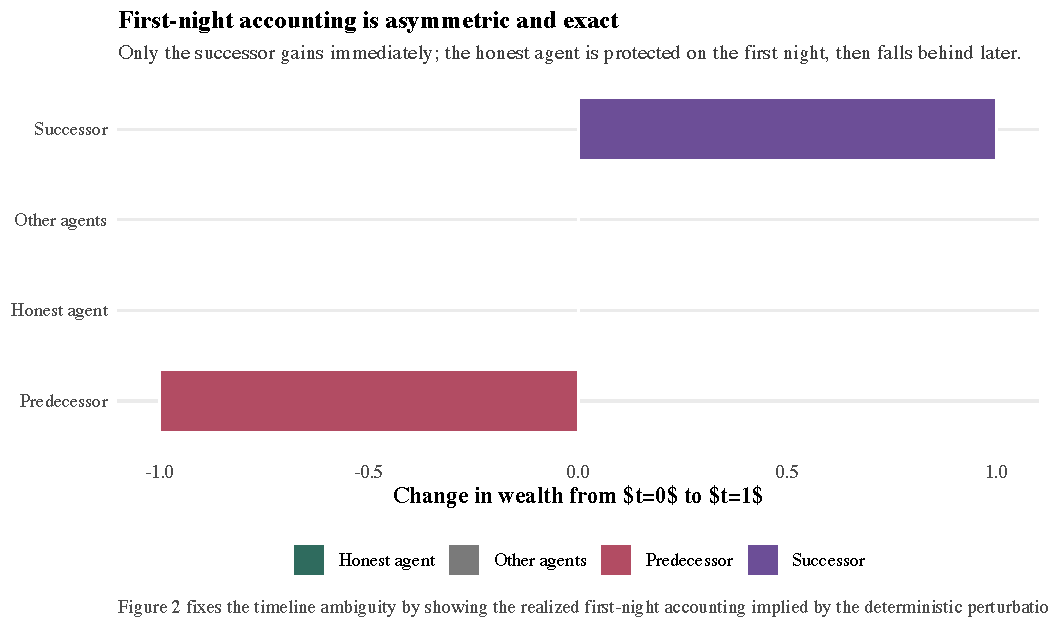
\includegraphics[width=\mediumfigwidth]{figures/fig02_first_night_accounting.pdf}
    \caption{First night accounting. The honest agent is protected on the first night and is robbed only later in the transition, so the winner and loser on that night are the successor and predecessor in the original cycle. This timeline underlies the instability theorem.}
    \label{fig:fig02_first_night_accounting}
\end{figure}

The deterministic environment leaves no room to attribute the departure from the original cycle to chance. Once successor wealth exceeds the threshold in \eqref{eq:threshold}, the continuation path begins to involve further choices to stay home and new interruptions in the network. The event time display therefore traces the mechanism stated in Theorem \ref{thm:no-stationary-one-honest} in realized form.

\subsection{From local asymmetry to class formation}

Longer horizon simulations show that the honest shock generates persistent class structure that survives well beyond the initial reshuffling of positions. Figure \ref{fig:fig03_event_time_roles} groups agents by the highest institutional role they reach during the transition and traces the corresponding wealth paths in event time, a grouping that preserves the early separation because many agents later withdraw into staying or inactivity. Agents who eventually become patrons pull away almost immediately after the initial disturbance, agents who later serve as guards remain well below them, and the honest household falls away sharply. Differentiation therefore begins before the late path settles into a quieter occupational pattern, in line with the theory that rich households emerge first because personal exposure changes the occupational choice of early windfall recipients and patronage enters only after that distribution has already begun to separate.

\begin{figure}[tbp]
    \centering
    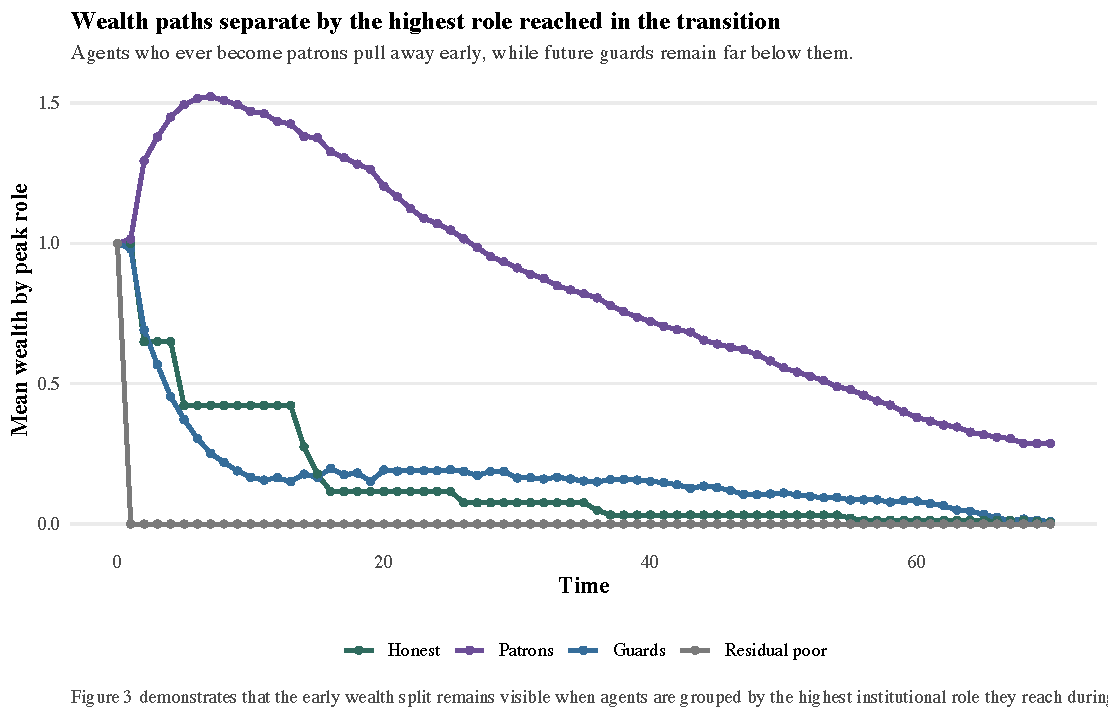
\includegraphics[width=\mainfigwidth]{figures/fig03_event_time_roles.pdf}
    \caption{Event time wealth trajectories by peak role in the transition. Agents who ever become patrons separate quickly from future guards and the residual poor. Class differentiation appears early in the transition and does not depend on the terminal date.}
    \label{fig:fig03_event_time_roles}
\end{figure}

Figure \ref{fig:fig04_distribution_evolution} shows the same process in cross section. The heatmap and quantile ribbons reveal a distribution that rapidly loses its middle. In early periods the support remains narrow because the honest perturbation is still local. A few periods later the upper tail thickens while the lower quantiles bend downward as repeated raids and weak outside options trap a growing mass of agents in the poor set. The widening is not symmetric. The upper tail is carried by a small number of agents who stop exposing their own wealth and later capture part of delegated loot, while the lower tail contains agents who continue to circulate through risky occupations and increasingly depleted target pools. The simulation is therefore producing more than heterogeneity. It is producing a different allocation of risk, power, and occupational choice across the distribution.

\begin{figure}[tbp]
    \centering
    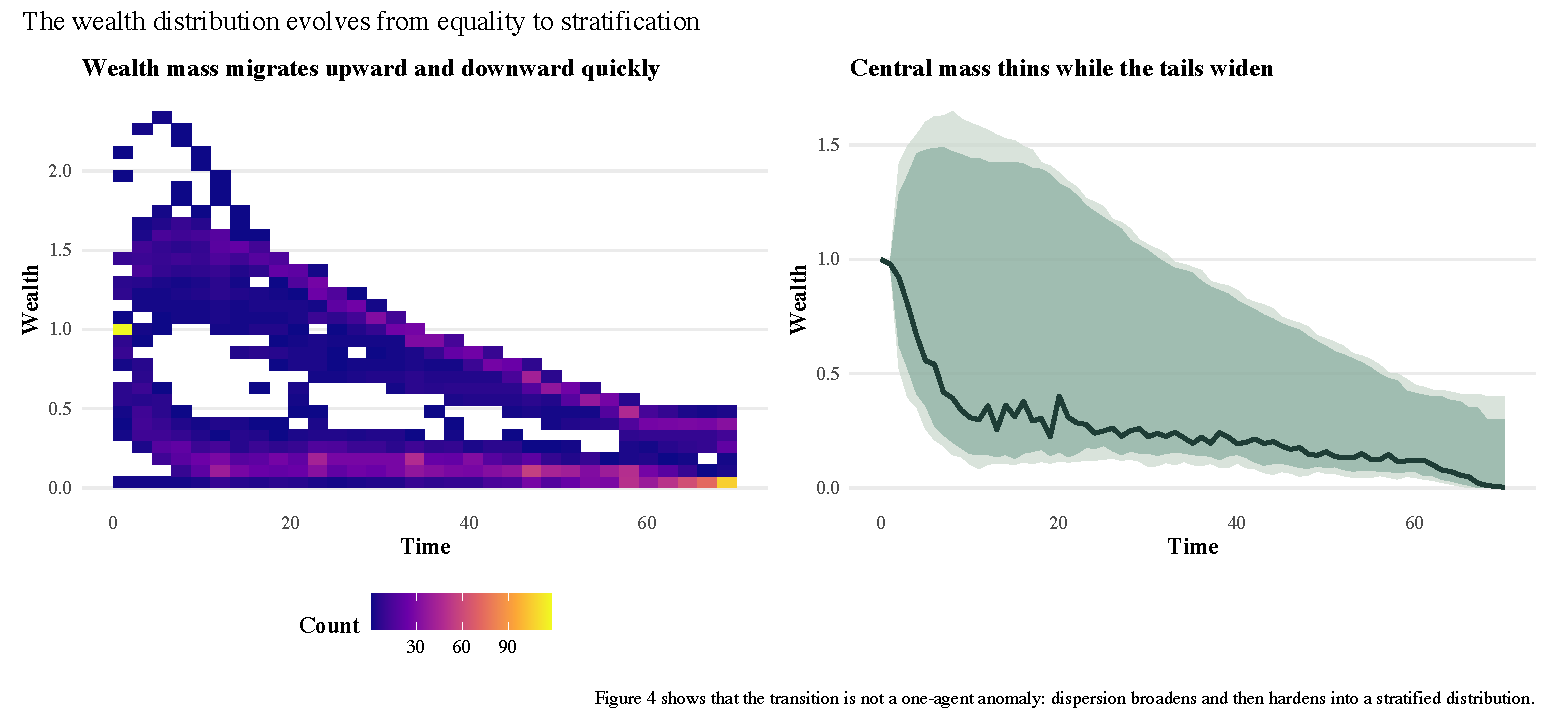
\includegraphics[width=\mainfigwidth]{figures/fig04_distribution_evolution.pdf}
    \caption{Evolution of the wealth distribution. The heatmap and quantile bands show the rapid thinning of the middle and the thickening of both tails. The honest perturbation produces durable stratification instead of a temporary reshuffle.}
    \label{fig:fig04_distribution_evolution}
\end{figure}

Figure \ref{fig:fig05_inequality_dynamics} translates that cross sectional movement into conventional distributional statistics. The Gini coefficient rises sharply from its benchmark value near zero. The top decile wealth share increases in tandem. Lorenz curves at selected dates move steadily away from the forty five degree line. The summary statistics matter because they show that the transition is not confined to a few pathwise anecdotes. The distributional consequences are large, systematic, and persistent in the baseline calibration.

\begin{figure}[tbp]
    \centering
    
\includegraphics[width=\mainfigwidth]{figures/fig05_inequality_dynamics.pdf}
    \caption{Inequality dynamics. The Gini coefficient, top decile wealth share, and Lorenz curves all move sharply away from the egalitarian benchmark. The transition has strong and persistent distributional consequences.}
    \label{fig:fig05_inequality_dynamics}
\end{figure}

These displays show a determinate sequence from local perturbation to durable inequality. The deterministic shock creates a state difference, the exposure threshold turns that difference into differentiated behavior, and the proportional environment amplifies the behavioral split because rich households internalize exposure while poor households remain available for predatory labor. The simulated path therefore gives the theoretical sequence visible economic content instead of leaving it as an abstract transition argument.

\subsection{Patronage and the surplus from delegation}

Across an interpretable range of parameters, rich agents hire poor thieves only when the contract creates surplus that is both feasible and privately valuable. Figure \ref{fig:fig06_contracting_comparative_statics} examines that condition directly. The left panel varies the targeting advantage of delegation. The right panel traces the gap between compensation and the outside option as worker slackness changes. Patron surplus rises with the first margin and falls as the second margin strengthens, exactly as Proposition \ref{prop:patronage} predicts. Delegated theft that is better targeted than freelancing leaves room to satisfy participation and still retain a positive residual. A stronger outside option narrows that residual and can eliminate it.

\begin{figure}[tbp]
    \centering
    
\includegraphics[width=\mainfigwidth]{figures/fig06_contracting_comparative_statics.pdf}
    \caption{Contracting comparative statics. Patron surplus rises when delegated theft has a stronger targeting advantage and poor outside options are weaker. The source of patron surplus is explicit, and the earlier zero profit knife edge disappears.}
    \label{fig:fig06_contracting_comparative_statics}
\end{figure}

Delegation becomes profitable only because the environment generates a clear wedge between delegated returns and the outside option of the thief. If the thief could always obtain alone the same gross loot he could obtain for the patron, and if the patron had neither targeting advantage nor bargaining power, patronage would collapse to a zero-profit transfer. Here the patron directs predation more effectively or protects the contract well enough to make delegation more productive than freelancing, while the thief operates in a crowded and depleted market. The gap between delegated returns and the outside option pays the contracting cost and still leaves a residual for the patron.

Patronage need not be monotone in every parameter that raises expected loot. When theft intensity becomes too large, the prey base can be depleted quickly, which shortens the durability of the contract regime even when delegation is initially attractive. Proposition \ref{prop:patronage} gives the static dominance condition; the simulations trace its interaction with depletion, competition, and regime duration.

\subsection{From patronage to guarding}

Figure \ref{fig:fig07_regime_phase_diagram} maps the dominant medium run regime over the parameter plane spanned by theft intensity and enforcement effectiveness. Low theft intensity combined with weak enforcement tends to preserve a long transition because the returns to both predation and protection remain limited. As theft intensity rises and enforcement becomes more effective, the dominant regime shifts toward coexistence and guarding. Collapse appears where predation is intense enough and protection weak enough that the social base is depleted before a stable protected elite can consolidate. The pattern matches the logic of Theorem \ref{thm:guarding}: once concentrated wealth becomes valuable enough to protect and protection becomes sufficiently effective, elites preserve existing claims instead of financing one more round of delegated extraction.

\begin{figure}[tbp]
    \centering
    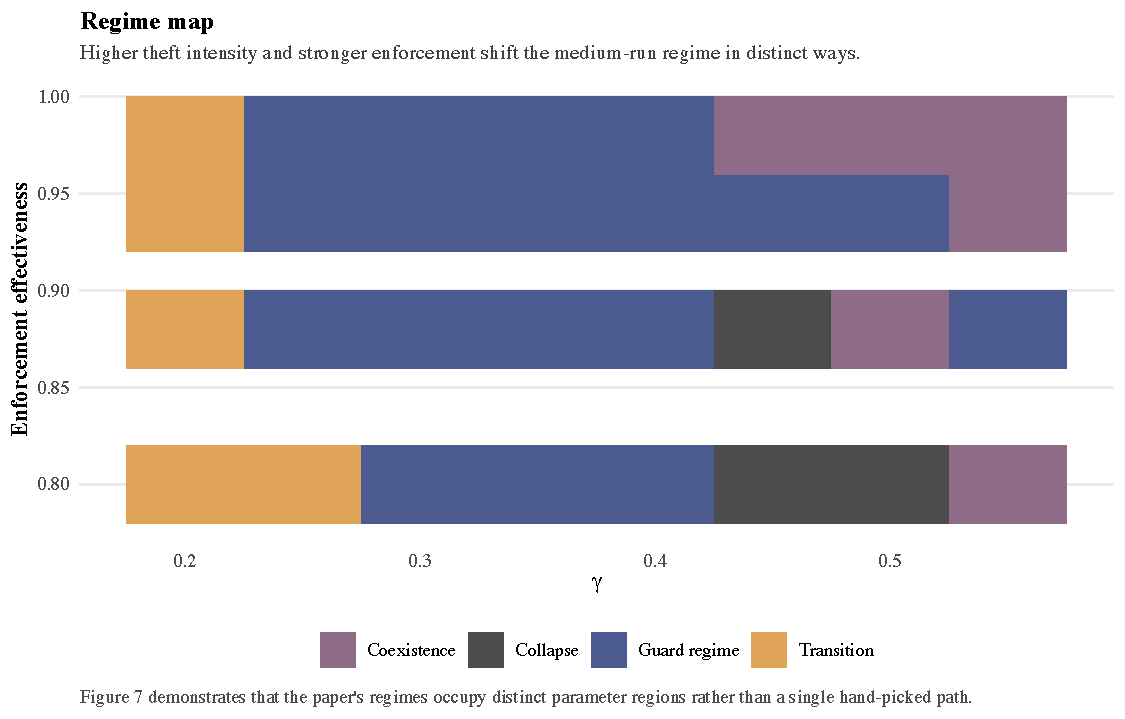
\includegraphics[width=\mediumfigwidth]{figures/fig07_regime_phase_diagram.pdf}
    \caption{Regime phase diagram. Different combinations of theft intensity and enforcement effectiveness lead to distinct medium run transition, coexistence, guard, and collapse regions. The successor regimes occupy distinct and interpretable parts of the parameter space.}
    \label{fig:fig07_regime_phase_diagram}
\end{figure}

On this parameter plane, patronage appears mainly as a transitional corridor and only infrequently as the dominant medium run regime. The diagram is therefore populated mostly by transition, coexistence, guard, and collapse regions, even though patronage remains visible in the event time paths, network snapshots, and contracting comparative statics. The phase diagram adds an important qualification: delegation can organize the middle of the transition without remaining the dominant institutional form once enforcement becomes effective or depletion becomes severe.

Figure \ref{fig:fig08_role_shares} restores time to the same regime logic. The share of agents engaged in direct or freelance theft falls after the first perturbation. Patrons and hired thieves rise next. Guards appear later and remain active through much of the enforcement phase, even though their share is not monotone over time. The plot works as an occupational decomposition of the whole mechanism. The early decline in universal theft reflects the exposure logic of Theorem \ref{thm:no-stationary-one-honest}. The rise in patron and hired thief roles reflects the surplus logic of Proposition \ref{prop:patronage}. The later appearance of guarding reflects the threshold logic of Theorem \ref{thm:guarding}.

\begin{figure}[tbp]
    \centering
    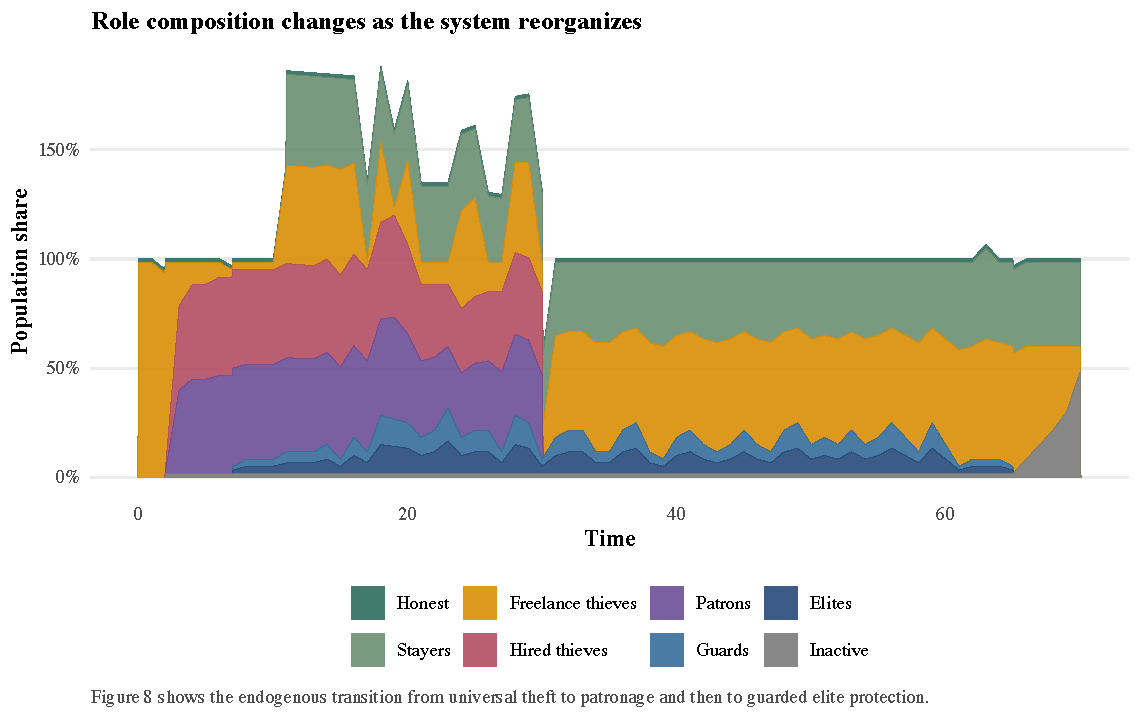
\includegraphics[width=\mainfigwidth]{figures/fig08_role_shares.pdf}
    \caption{Role shares over time. Universal theft gives way first to patronage and later to selective protection, with guarding remaining present through much of the enforcement phase. The social hierarchy reorganizes endogenously after the first honest shock.}
    \label{fig:fig08_role_shares}
\end{figure}

Figure \ref{fig:fig09_transition_timing} separates the part of the transition pinned down by chronology from the part left open by subsequent state evolution. Under the simulation timing, the first opportunity to hire arrives immediately after the deterministic honest shock, and every run generates at least one patron at that first post-shock contracting round, so a raw first-entry statistic for patronage carries little information. The left panel therefore measures the scale of the patronage complex at time $3$, after the first hiring cascade has unfolded, while the right panel records the date at which guards reach five percent of the population. Broader honest shocks do not produce a smooth one for one acceleration in this clustered shock sweep because enlarging the initial honest set changes the local geometry of the broken cycle as well as its size. The picture that remains is immediate reorganization into patronage followed by a later and more dispersed movement into enforcement once wealth concentration and prey depletion have advanced far enough.

\begin{figure}[tbp]
    \centering
    
\includegraphics[width=\mainfigwidth]{figures/fig09_transition_timing.pdf}
    \caption{Early patronage and later guard timing. The first patron appears at the earliest feasible post-shock contracting round in every run, so the left panel reports the share of patrons and hired thieves at time $3$. The right panel reports the time at which guards reach five percent of the population. Organizational change is immediate after the honest shock, while movement into enforcement arrives later and with more dispersion.}
    \label{fig:fig09_transition_timing}
\end{figure}

Coexistence reveals institutional layering instead of a synchronized regime switch. In those paths, some elites have crossed the guard threshold while others still rely on patronage, so different technologies of control operate at the same time in different parts of the wealth distribution. The move from patronage to guarding is therefore unequal and sequential: some elites buy security before others can and stabilize their lead in the process.

Table \ref{tab:simulation-summary} compresses the same sequence across the baseline perturbation, patronage, and enforcement simulations after the timing, regime, and occupational evidence is in place. The baseline perturbation is the least unequal of the three simulated environments. Patronage produces a larger rise in concentration because it adds a contract technology that channels loot upward. Enforcement then preserves and slightly intensifies that concentration. In this sense the table mirrors Proposition \ref{prop:welfare}: distributional divergence is already visible once reciprocity breaks, and later regimes magnify that divergence or lock it in through new organizational choices.

\begin{table}[tbp]
    \centering
    \caption{Simulation summary. The first honest perturbation produces a local distributional break, patronage transforms that break into durable stratification, and enforcement preserves or deepens concentrated wealth instead of reversing it.}
    \label{tab:simulation-summary}
    \begin{tabular}{lcccll}
\toprule
Scenario & Gini & Top decile & First patron & First guard & Regime \\
\midrule
Baseline perturbation & 0.231 & 0.200 & Not reached & Not reached & Transition \\
Patronage dynamics & 0.575 & 0.296 & 2 & Not reached & Transition \\
Enforcement dynamics & 0.640 & 0.306 & 2 & 7 & Guard regime \\
\bottomrule
\end{tabular}

\end{table}

\subsection{Network reorganization and welfare}

Figure \ref{fig:fig10_network_snapshots} makes the organizational change visible in network form. On the first honest night the graph is still dominated by direct theft edges arranged around the original cycle. In the middle snapshot, contract links connect patrons to hired thieves and theft edges point from those thieves toward vulnerable poor households. In the later snapshot, guard links radiate from elite households while direct theft edges thin out. The pattern of social linkage changes along with the wealth distribution, as horizontal predation gives way to vertical contracting and then to selective protection.

\begin{figure}[tbp]
    \centering
    
\includegraphics[width=\mainfigwidth]{figures/fig10_network_snapshots.pdf}
    \caption{Network snapshots across regimes. Direct theft edges dominate at first, contract edges later connect patrons to thieves, and guard edges eventually organize elite protection. The network structure of predation and control changes with the regime.}
    \label{fig:fig10_network_snapshots}
\end{figure}

Figure \ref{fig:fig11_welfare_decomposition} reports the welfare consequences of the transition. Gross wealth and utilitarian welfare do not move together. Aggregate wealth declines steadily because theft, punishment, and protection burn resources even when much of the interaction is redistributive in form. Welfare deteriorates more sharply because redistribution toward the top lowers the concave utility sum and because predation, contracting, punishment, and guarding all consume resources. Proposition \ref{prop:welfare} formalizes this mechanism. Low welfare in the transition comes from the unequal and resource consuming adjustment that follows an incomplete honest shock.

\begin{figure}[tbp]
    \centering
    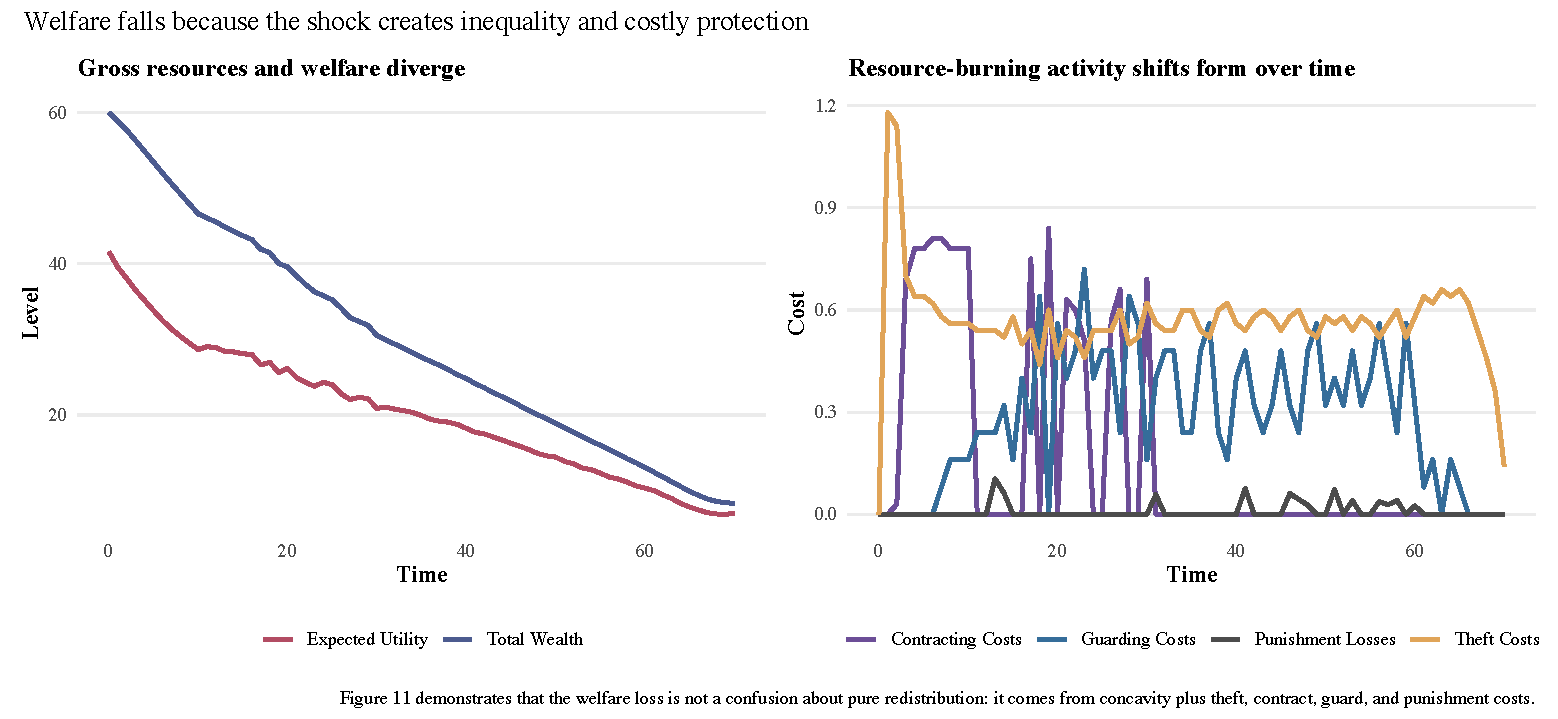
\includegraphics[width=\mainfigwidth]{figures/fig11_welfare_decomposition.pdf}
    \caption{Welfare decomposition. Aggregate wealth and utilitarian welfare diverge because the transition adds inequality and resource burning activity in the form of theft, contracts, punishment, and guarding. The welfare mechanism appears directly in the decomposition.}
    \label{fig:fig11_welfare_decomposition}
\end{figure}

Because Figure \ref{fig:fig11_welfare_decomposition} follows one baseline enforcement path rather than a comparison across parameter regions, its most direct contribution lies in the composition of resource use over time. Theft costs dominate early, contracting costs spike during patronage, and guarding costs remain persistent later on. Guard adoption changes how resources are burned without restoring the earlier welfare level, and the protected order that emerges at the end still rests on concentrated wealth accumulated during the predatory transition.

\subsection{Robustness}

Figure \ref{fig:fig12_robustness_panels} collects the main one dimensional robustness exercises in compact form. Final welfare responds most strongly to theft intensity and occupied house vulnerability in this sweep, while final inequality moves within a narrower band. Regime classification also changes little once the system is already in the region where guarding is attractive. Among the four margins shown, only the theft intensity sweep changes the dominant regime, passing from transition to guard and then to coexistence as extraction becomes harsher. The other sweeps mainly alter the severity of the outcome. The panels therefore indicate a mechanism that survives beyond a single calibration, even though some margins move welfare far more than they move regime labels.

\begin{figure}[tbp]
    \centering
    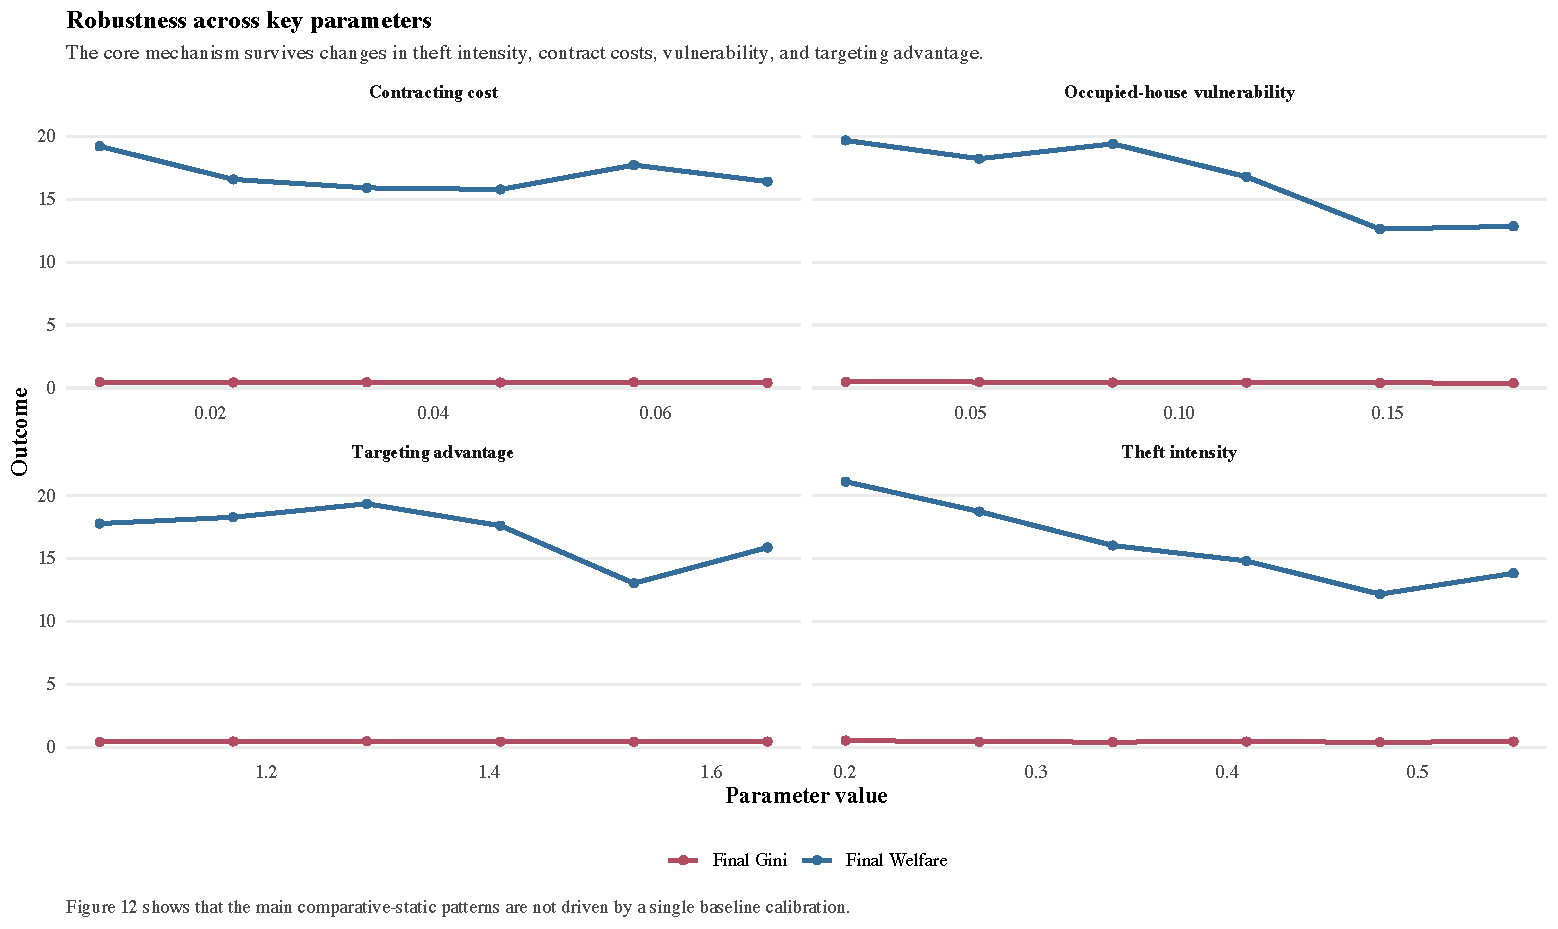
\includegraphics[width=\mainfigwidth]{figures/fig12_robustness_panels.pdf}
    \caption{Robustness panels. The top row reports final inequality, the bottom row reports final welfare, and point markers identify the dominant regime reached at each parameter value. The mechanism survives beyond a single calibration, although some margins move welfare more than regime labels.}
    \label{fig:fig12_robustness_panels}
\end{figure}

The failure cases identify the conditions under which the mechanism attenuates. High contracting costs and weak targeting advantage compress delegation surplus, while low occupied house vulnerability reduces the value of moving from mere presence to organized protection. The sweeps therefore locate the margins that mute the transition without suggesting that every one dimensional variation redraws the institutional map.

Figure \ref{fig:fig07_regime_phase_diagram} is the more informative display for collapse. There the collapse cells do not mark a numerical artifact or a moral inversion of balanced reciprocity. They identify paths in which predation and protection together destroy the social base that made them profitable. Poor households become too depleted to sustain patronage, and inequality becomes so sharp that a small protected core cannot reorganize the rest into a stable order. This possibility prevents the model from telling a falsely deterministic story in which every corrupt equilibrium matures smoothly into guarded hierarchy.

\section{Discussion and Conclusion}
\label{sec:discussion}

The sequence developed here isolates a form of order that remains stable while saturated with predation. Equality survives there only in the thin accounting sense that every loss is offset by a corresponding gain, and once that accounting is disturbed the successor need not be cleaner, more egalitarian, or morally mixed in any interesting way. It can instead become a harder arrangement in which the distribution created during the transition is defended more effectively than it was created. The stages of that movement remain distinct: balanced reciprocity governs the unit benchmark, a permanent honest perturbation destroys stationarity once exposure becomes wealth dependent, delegated predation emerges when wealth and vulnerability diverge enough to create surplus from hiring, and organized protection arrives when concentrated wealth becomes worth defending and the prey base has already been thinned. Welfare follows the same sequence. Honesty does not become socially harmful; welfare falls because a local rupture in a corrupt equilibrium is followed by unequal adjustment when no broader institutional change accompanies it. Some agents reduce exposure by staying home, then by hiring thieves, and later by hiring guards, while others become more exposed as their outside options weaken with repeated loss. Concavity in wealth, theft effort costs, contracting costs, guarding costs, and punishment losses all move in the same direction.

Guards and police appear only after concentrated wealth has become worth protecting and labor can be shifted from predation to protection without altering who controls the terms of social order. The move to guarding therefore replaces one order with another; it does not mark the first appearance of order. Simulation is useful precisely because that replacement unfolds through state dependence that is hard to characterize in closed form once many heterogeneous agents interact: exact event time makes the first honest night visible, patronage and enforcement paths show how the payoff comparisons behave after symmetry has broken, and the phase diagram together with the robustness panels show where the mechanism survives and where it gives way to coexistence or collapse. Production is absent, so the analysis concerns the redistribution, dissipation, and protection of wealth rather than its endogenous creation, and the final regime remains protection of accumulated spoils rather than a full productive property-rights order. The case studied is also the one that gives the fable its force, namely a small honest rupture inside a society whose predatory balance relied on universal participation, while a broader coalition of honest agents could generate a different transition.

The paradox that made the story worth modeling remains: universal theft can look balanced, honesty can break that balance without redeeming the society, and the calmer order that follows can also be the more unequal order. Those claims now rest on explicit conditions. A balanced theft cycle can persist under symmetry, a permanent honest perturbation destroys stationarity once exposure becomes wealth dependent, patronage requires surplus over poor outside options, and guarding becomes privately optimal once concentrated wealth and prey depletion change the ranking of control technologies. The computational evidence completes the sequence by showing a precise first night asymmetry, a durable widening of the distribution, a contract regime grounded in explicit surplus, and a later move toward protection that stabilizes gains accumulated during the predatory transition. Calvino remains central because the story locates the whole movement with unusual economy.

\section*{Acknowledgements}

The author thanks readers of earlier drafts for comments that sharpened the argument and exposed several formal ambiguities in the first version. No external funding supported this research.

\section*{Declaration of Competing Interest}

The author declares no known competing financial interests or personal relationships that could have appeared to influence the work reported in this article.

\section*{Data Availability}

All code, generated simulation outputs, and build scripts required to reproduce the figures and tables are available in the project repository at \href{https://github.com/cheikh-a/black_sheep_geb}{github.com/cheikh-a/black\_sheep\_geb}. A versioned archival release can be deposited at the time of publication if the journal requests a persistent repository record.

\section*{Declaration of Generative AI and AI-assisted Technologies in the Writing Process}

Generative AI and AI-assisted tools were used under author supervision during revision of the manuscript to support language editing, code debugging, figure-production scripting, and consistency checks. All theoretical claims, modeling choices, simulations, interpretations, and editorial decisions were reviewed and approved by the author, who takes full responsibility for the content of the article.


\bibliographystyle{plainnat}
\bibliography{refs}

\appendix
\section{Appendix}

\subsection{Proofs}
\label{app:proofs}

This appendix collects the proof details omitted from the main text. None of the omitted steps is especially difficult. The purpose of placing them here is simply to keep the main text readable while making the logical dependence of the results explicit. Throughout, the benchmark unit loot is $\tau = 1$ unless otherwise noted.

\subsubsection*{Proof of Lemma \ref{lem:balanced-accounting}}

Fix a balanced theft cycle $\sigma$ and suppose every agent enters the period with wealth $\bar{w}$. By definition of a balanced cycle, each household is unoccupied and is targeted by exactly one raider, so $m_{jt}=1$ for every $j$. Equation \eqref{eq:loss-gain} therefore implies $\ell_{it}(a_t)=\tau$ and $g_{it}(a_t)=\tau$ for every agent $i$. Equation \eqref{eq:benchmark-wealth-update} becomes
\[
w_{i,t+1} = \bar{w} - \tau + \tau = \bar{w}
\]
for every agent $i$. Summing across agents yields
\[
\sum_{i=1}^{N} w_{i,t+1} = \sum_{i=1}^{N} \bar{w} = N \bar{w} = \sum_{i=1}^{N} w_{it}.
\]
Hence wealth is preserved both agent by agent and in aggregate. \qed

\subsubsection*{Proof of Proposition \ref{prop:balanced-cycle}}

Take an arbitrary agent $i$ in a balanced theft cycle. If $i$ follows the prescribed action, then $i$ leaves home, loses $\tau$ to the unique incoming raid, and gains $\tau$ from the unique outgoing raid, finishing with wealth $\bar{w}$.

If $i$ deviates to staying home, the incoming raid on $i$ fails because the house is occupied, but $i$ also gives up the outgoing loot. The deviating payoff is therefore still $\bar{w}$, so staying home is not strictly profitable.

If instead $i$ deviates to another target $j \neq \sigma(i)$, then household $j$ is already targeted by exactly one raider under the balanced cycle. The deviator therefore creates congestion at $j$ and receives expected loot $\tau/2$ rather than $\tau$. The incoming raid on $i$ still succeeds because $i$ remains away from home. The deviating payoff is then
\[
\bar{w} - \tau + \frac{\tau}{2}
=
\bar{w} - \frac{\tau}{2}
<
\bar{w}.
\]
Thus every retargeting deviation is strictly worse, while staying home is payoff equivalent. No unilateral deviation is strictly profitable, so the balanced cycle is a weak Nash equilibrium. \qed

\subsubsection*{Proof of Lemma \ref{lem:first-night}}

Let $h$ be the permanently honest agent, $p = \sigma^{-1}(h)$ his predecessor in the original cycle, and $q = \sigma(h)$ his successor. At $t=0$, agent $h$ stays home. Because occupied houses cannot be burgled in the benchmark environment, the raid by $p$ against $h$ fails, so $p$ gains no loot from his planned target. Agent $h$ also undertakes no outgoing raid, so $q$ is not robbed by $h$. All other agents follow the original cycle exactly.

Now compute end-of-night wealth. Agent $h$ neither loses nor gains, so $w_{h1} = \bar{w}$. Agent $p$ is still robbed by his own predecessor but gains nothing from his failed attempt on $h$, so $w_{p1} = \bar{w} - \tau$. Agent $q$ still robs his own target but is no longer robbed by $h$, so $w_{q1} = \bar{w} + \tau$. Every other agent both loses $\tau$ and gains $\tau$, hence remains at $\bar{w}$. This proves \eqref{eq:first-night-accounting}. \qed

\subsubsection*{Proof of Theorem \ref{thm:no-stationary-one-honest}}

By Lemma \ref{lem:first-night}, the successor $q$ enters period $t=1$ with wealth $w_{q1} = \bar{w} + \tau$. The expected one period net payoff from personal theft at wealth $w$ is
\[
\pi^{S}(w) = \tau - \rho w - c_T.
\]
The payoff from staying home is normalized to zero. Therefore the agent strictly prefers staying home whenever $w > \widehat{w} = (\tau - c_T)/\rho$.

Assumption \ref{ass:threshold} states that $\bar{w} < \widehat{w} < \bar{w} + \tau$. The lower inequality ensures that at the symmetric benchmark wealth level $\bar{w}$ an agent weakly prefers theft or is indifferent, which is why the original cycle can be sustained before the honest perturbation. The strict upper inequality ensures that after the first-night windfall the successor's wealth lies strictly above the cutoff. Hence
\[
\pi^{S}(w_{q1})
=
\tau - \rho(\bar{w}+\tau) - c_T
<
\tau - \rho\widehat{w} - c_T
=
0
\]
so staying home is strictly better for the successor at state $w_{q1}$.

To prove the theorem as stated, suppose by contradiction that there exists a stationary Markov equilibrium preserving the original balanced theft pattern among all nonhonest agents. Then $q$ must choose personal theft at state $w_{q1}$. But the threshold condition implies that staying home strictly dominates personal theft at exactly that state. This contradicts the alleged stationary continuation. Therefore no such stationary Markov equilibrium exists. \qed

\subsubsection*{Proof of Lemma \ref{lem:contract-feasibility}}

Fix a rich patron $i$ and a candidate poor thief $j$. Let delegated gross loot be $L_t$, contracting cost $k$, and the outside option of the poor worker $o_{jt}$. A contract with terms $(s_{ijt}, \alpha_{ijt})$ is feasible if the participation constraint of the thief holds:
\[
s_{ijt} + \alpha_{ijt}L_t \ge o_{jt}.
\]
The net return of the patron from the contract is
\[
(1-\alpha_{ijt})L_t - s_{ijt} - k = L_t - \left(s_{ijt} + \alpha_{ijt}L_t\right) - k.
\]
For some contract to be mutually acceptable, there must exist a transfer to the thief that is at least $o_{jt}$ and leaves the patron weakly nonnegative. This requires
\[
o_{jt} \le s_{ijt} + \alpha_{ijt}L_t \le L_t - k.
\]
Such an interval exists if and only if $L_t - k - o_{jt} \ge 0$, with strict inequality for strictly positive joint surplus. This is exactly condition \eqref{eq:feasibility}. \qed

\subsubsection*{Proof of Proposition \ref{prop:patronage}}

Suppose \eqref{eq:feasibility} holds, so total joint surplus is
\[
\Sigma_t = L_t - k - o_{jt} > 0.
\]
Under the bargaining rule in \eqref{eq:bargaining-rule}, the thief receives
\[
o_{jt} + (1-\beta)\Sigma_t
\]
in expected value, while the patron receives the residual
\[
L_t - k - \left[o_{jt} + (1-\beta)\Sigma_t\right]
 = L_t - k - o_{jt} - (1-\beta)\Sigma_t
 = \beta \Sigma_t.
\]
This proves \eqref{eq:patron-payoff}. Hiring dominates abstention whenever $\beta \Sigma_t > 0$, and it dominates personal theft whenever
\[
\beta \Sigma_t > m_t - \rho w_{it} - c_T.
\]
Combining the two comparisons yields \eqref{eq:patron-dominance}. \qed

\subsubsection*{Proof of Corollary \ref{cor:patronage-statics}}

Using \eqref{eq:patron-payoff} together with $L_t = \phi_t \gamma \bar{w}^{H}_t$ and $o_{jt} = \lambda_t \gamma \bar{w}^{P}_t - c_T$, patron payoff can be written as
\[
\pi^{\mathrm{hire}}_{ijt}
=
\beta\left(\phi_t \gamma \bar{w}^{H}_t - k - \lambda_t \gamma \bar{w}^{P}_t + c_T\right).
\]
Differentiating yields
\[
\frac{\partial \pi^{\mathrm{hire}}_{ijt}}{\partial \phi_t}
=
\beta \gamma \bar{w}^{H}_t > 0,
\qquad
\frac{\partial \pi^{\mathrm{hire}}_{ijt}}{\partial \lambda_t}
=
- \beta \gamma \bar{w}^{P}_t < 0,
\qquad
\frac{\partial \pi^{\mathrm{hire}}_{ijt}}{\partial k}
=
-\beta < 0.
\]
Thus patron payoff rises with delegation quality and falls with poor outside options and contracting cost. Since patronage is chosen when \eqref{eq:patron-dominance} holds, any change that raises the left-hand side of that inequality, holding the right-hand side fixed, expands the set of states in which patronage dominates. \qed

\subsubsection*{Proof of Theorem \ref{thm:guarding}}

Elite agent $i$ compares the payoff from guarding,
\[
\pi^{\mathrm{guard}}_{it} = q_t \chi_t \gamma_E w_{it} - g,
\]
with the payoff from one more patron-thief contract,
\[
\pi^{\mathrm{hire}}_{ijt} = \beta\left(L_t - k - o_{jt}\right).
\]
Guarding is optimal if and only if
\[
q_t \chi_t \gamma_E w_{it} - g \ge \beta\left(L_t - k - o_{jt}\right),
\]
which rearranges to
\[
w_{it} \ge \frac{\beta\left(L_t - k - o_{jt}\right)+g}{q_t \chi_t \gamma_E} \equiv \widehat{w}^{G}_t.
\]
This proves the threshold expression in \eqref{eq:guard-threshold}. To show that the threshold falls as the poor prey base is depleted, note that both $L_t = \phi_t \gamma \bar{w}^{H}_t$ and $o_{jt} = \lambda_t \gamma \bar{w}^{P}_t - c_T$ depend positively on the wealth of the poor. Under the maintained assumption that delegated targeting advantage shrinks more slowly than the broad poor outside option, depletion lowers net delegated surplus $L_t - o_{jt}$ and hence lowers the threshold wealth level at which guarding dominates. \qed

\subsubsection*{Proof of Corollary \ref{cor:guard-statics}}

Write the guarding threshold as
\[
\widehat{w}^{G}_t
=
\frac{\beta(L_t-k-o_{jt}) + g}{q_t \chi_t \gamma_E}.
\]
Direct differentiation gives
\[
\frac{\partial \widehat{w}^{G}_t}{\partial q_t}
=
-\frac{\beta(L_t-k-o_{jt}) + g}{q_t^2 \chi_t \gamma_E} < 0,
\qquad
\frac{\partial \widehat{w}^{G}_t}{\partial \chi_t}
=
-\frac{\beta(L_t-k-o_{jt}) + g}{q_t \chi_t^2 \gamma_E} < 0,
\]
\[
\frac{\partial \widehat{w}^{G}_t}{\partial \gamma_E}
=
-\frac{\beta(L_t-k-o_{jt}) + g}{q_t \chi_t \gamma_E^2} < 0,
\qquad
\frac{\partial \widehat{w}^{G}_t}{\partial g}
=
\frac{1}{q_t \chi_t \gamma_E} > 0.
\]
Finally,
\[
\frac{\partial \widehat{w}^{G}_t}{\partial \{\beta(L_t-k-o_{jt})\}}
=
\frac{1}{q_t \chi_t \gamma_E} > 0.
\]
Hence stronger guarding technology or greater elite vulnerability lowers the wealth threshold for protection, while more profitable patronage or more expensive guard labor raises it. \qed

\subsubsection*{Proof of Proposition \ref{prop:welfare}}

Fix date $t$ and suppose aggregate wealth $\sum_i w_{it}$ is fixed. Let $u$ be concave. If one wealth vector is a mean preserving spread of another, then by the Hardy-Littlewood-Polya majorization theorem, or equivalently by Jensen's inequality applied to pairwise spreads, the more unequal vector yields a weakly smaller value of $\sum_i u(w_{it})$. This proves the first claim.

Now compare two regimes with the same aggregate wealth. If one regime has weakly greater inequality, then its utility sum is weakly lower. If, in addition, at least one of the cost terms $n_t^{S}$, $n_t^{H}$, $n_t^{G}$, or $\Psi_t$ is strictly larger and none is smaller, then subtracting those costs from the already weakly smaller utility sum yields strictly lower period welfare $\mathcal{W}_t$. This proves the second claim. \qed

\subsubsection*{Proof of Corollary \ref{cor:guard-welfare}}

Fix the wealth distribution. The difference between period welfare under guarding and period welfare under patronage is
\[
\Delta \mathcal{W}_t
=
- g n_t^{G}
- c_T n_t^{S,\mathrm{guard}}
- k n_t^{H,\mathrm{guard}}
- \Psi_t^{\mathrm{guard}}
+ c_T n_t^{S,\mathrm{pat}}
+ k n_t^{H,\mathrm{pat}}
+ \Psi_t^{\mathrm{pat}}.
\]
If the reduction in theft effort cost, contracting cost, and punishment loss exceeds the new guard wage bill, then $\Delta \mathcal{W}_t > 0$. Since the wealth distribution is fixed by hypothesis, the utility term cancels. Hence guarding raises welfare relative to patronage under the stated condition. \qed

\subsection{Alternative assumptions and scope}

Several assumptions deserve comment because they determine both what the paper proves and what it leaves open. The first is the use of a unit transfer benchmark followed by a proportional transfer extension. A single proportional model could in principle have been used throughout. The difficulty is that the egalitarian balance at the beginning of the story by Calvino is most transparent when every successful raid transfers the same unit amount and every agent has exactly one incoming and one outgoing link. The benchmark therefore isolates the cycle cleanly. Once the paper turns to inequality and class formation, however, the unit transfer environment becomes too rigid because it cannot represent the idea that richer agents risk more by leaving home. The proportional extension is introduced at exactly that point and no earlier.

The second assumption concerns stationary Markov strategies in the honest-perturbation theorem. A reader might ask whether history-dependent punishments could sustain a one-honest continuation even after the first windfall. The answer may well be yes in some environments, but that is not the object of the theorem. The theorem isolates the local best-response logic that the simulation later implements. It says that once the wealth of the successor moves above the exposure threshold, the original cycle is not a stationary continuation. That is the appropriate statement for a paper interested in regime transition and not in the folk-theorem support of arbitrary histories.

The third assumption concerns the outside option of poor workers. The paper models it as weak because poor agents compete for a depleted set of vulnerable targets and because bargaining power is tilted toward patrons. One could instead model search frictions, repeated matching, or explicit auctioning of predatory labor. Any of those would add realism, but the key analytical requirement would remain the same: patronage must create a wedge between delegated gross returns and the best alternative available to poor workers. Without that wedge, the contract market has no surplus to divide.

The fourth assumption concerns guarding. In the model, guarding becomes attractive once occupancy alone no longer fully protects concentrated wealth after patronage weakens and poaching risk rises. This is summarized by the residual elite-risk term $\chi_t$. A more elaborate microfoundation could model betrayal by former hired thieves, explicit coordination among freelancers, or the public-good aspect of policing. The reduced form used here is meant only to capture the fact that highly concentrated wealth becomes worth defending with a more dedicated technology than merely staying home.

\subsection{Simulation implementation details}

The algorithm below maps the formal objects into the computational steps that generate the figures and tables. The code remains the authoritative implementation, but the written version keeps the appendix in the same notation as the model and simulation sections.

\begin{enumerate}[leftmargin=1.5em]
    \item Initialize $N$ agents with common wealth $\bar{w}$, assign the balanced theft permutation $\sigma$, and designate the initial honest set. In the baseline path the honest set contains one permanent honest agent.
    \item Run the deterministic benchmark perturbation. On the first night the honest agent stays home, all other agents follow the original cycle, and wealth is updated according to the accounting in Lemma \ref{lem:first-night}.
    \item In later benchmark periods, let each nonhonest agent compare current wealth to the threshold $\widehat{w}$ in \eqref{eq:threshold}. Agents above the threshold stay home; agents below it continue the cycle.
    \item For the proportional transfer simulations, reinitialize from the common wealth state and apply the first honest perturbation, then classify rich and elite agents each period using the threshold multipliers $\theta_R$ and $\theta_E$.
    \item Compute candidate personal theft returns for rich agents using \eqref{eq:personal-payoff}. Compute candidate contract surplus using \eqref{eq:total-surplus} and accept only contracts satisfying \eqref{eq:feasibility}. Order patrons from richest to poorest and match them to the poorest available workers, which is the code-level implementation of the offer stage in the extension game.
    \item Assign hired thieves to the high value poor target set $H_t$, freelancers to vulnerable households ranked by expected loot, and guards to elite households satisfying \eqref{eq:guard-threshold}. Apply the guard acceptance condition \eqref{eq:guard-IR}.
    \item Realize raids sequentially as the code-level counterpart to the rival-loot rule in \eqref{eq:success-probability}. Each realized transfer is based on the victim's remaining wealth at the moment of attack, so collisions on one house generate diminishing returns within a period.
    \item Apply wages, loot shares, contracting costs, guard wages, and punishment losses. Update the wealth vector and the role vector.
    \item Compute inequality statistics, welfare components, first entry times into patronage and guarding, and the regime label for the period. Store these outputs before advancing to the next date.
    \item Repeat until the simulation horizon is reached. Store processed data, figures, and tables through the reproducible build pipeline documented in the replication materials.
\end{enumerate}

Three implementation choices are especially important. First, wealth changes are recorded in realized rather than merely expected values, but the occupational comparisons are based on expected payoff formulas that correspond to the theory. Second, occupied but unguarded houses are treated differently in the first night benchmark and the later stochastic simulations. In the benchmark they are perfectly safe because that is what the instability theorem requires. In the later simulations they are imperfectly safe because concentrated wealth eventually requires a dedicated protection technology. Third, the code distinguishes clearly between rich households hiring poor thieves to rob poor targets and elites later hiring poor guards to defend elite assets. This distinction was blurred in the earlier draft and is now maintained throughout.

\subsection{Supplementary robustness and regime frequencies}

The phase diagram in the main text summarizes the most informative parameter plane, but the code evaluates broader robustness variations. These include changes in the outside option parameter, the number of initially honest agents, the guard punishment probability, and the vulnerability of occupied but unguarded homes. The overall message is the same as in the main text: the mechanism is robust within a substantial region, but it does not survive when the analytical conditions behind the main propositions are switched off. If delegated theft has no surplus, patronage disappears. If guarding is ineffective or too expensive, elites continue with patronage or the system collapses. If theft intensity is too low, the society can remain close to the transition regime for long periods.

Table \ref{tab:regime-frequencies} reports the frequency with which each dominant regime appears in the main parameter sweep. These frequencies are not structural predictions, because they depend on the chosen grid. Their value is descriptive. They show that transition, coexistence, guarding, and collapse all appear in the sweep, which confirms that the model generates multiple successor regimes and not a single canned trajectory.

\begin{table}[tbp]
    \centering
    \caption{Dominant regime frequencies in the main parameter sweep. The table reports how often each regime is the dominant late period outcome over the grid used to produce the phase diagram.}
    \label{tab:regime-frequencies}
    \begin{tabular}{lr}
\toprule
Dominant regime & Frequency \\
\midrule
Guard regime & 18 \\
Coexistence & 6 \\
Transition & 5 \\
Collapse & 3 \\
\bottomrule
\end{tabular}

\end{table}

\subsection{Annotated passage map for \emph{The Black Sheep}}

The translated story is not reproduced in full here because the text remains copyrighted. What can be included usefully is a passage map that identifies the parts of the story on which the model relies and the analytical object attached to each part. Figure \ref{fig:calvino-map} does that in paraphrased form.\footnote{The map is based on the sequence in \citet{calvino_1993}. It is intended as an interpretive guide to the model, not as a substitute for the story.}

\begin{figure}[tbp]
    \centering
    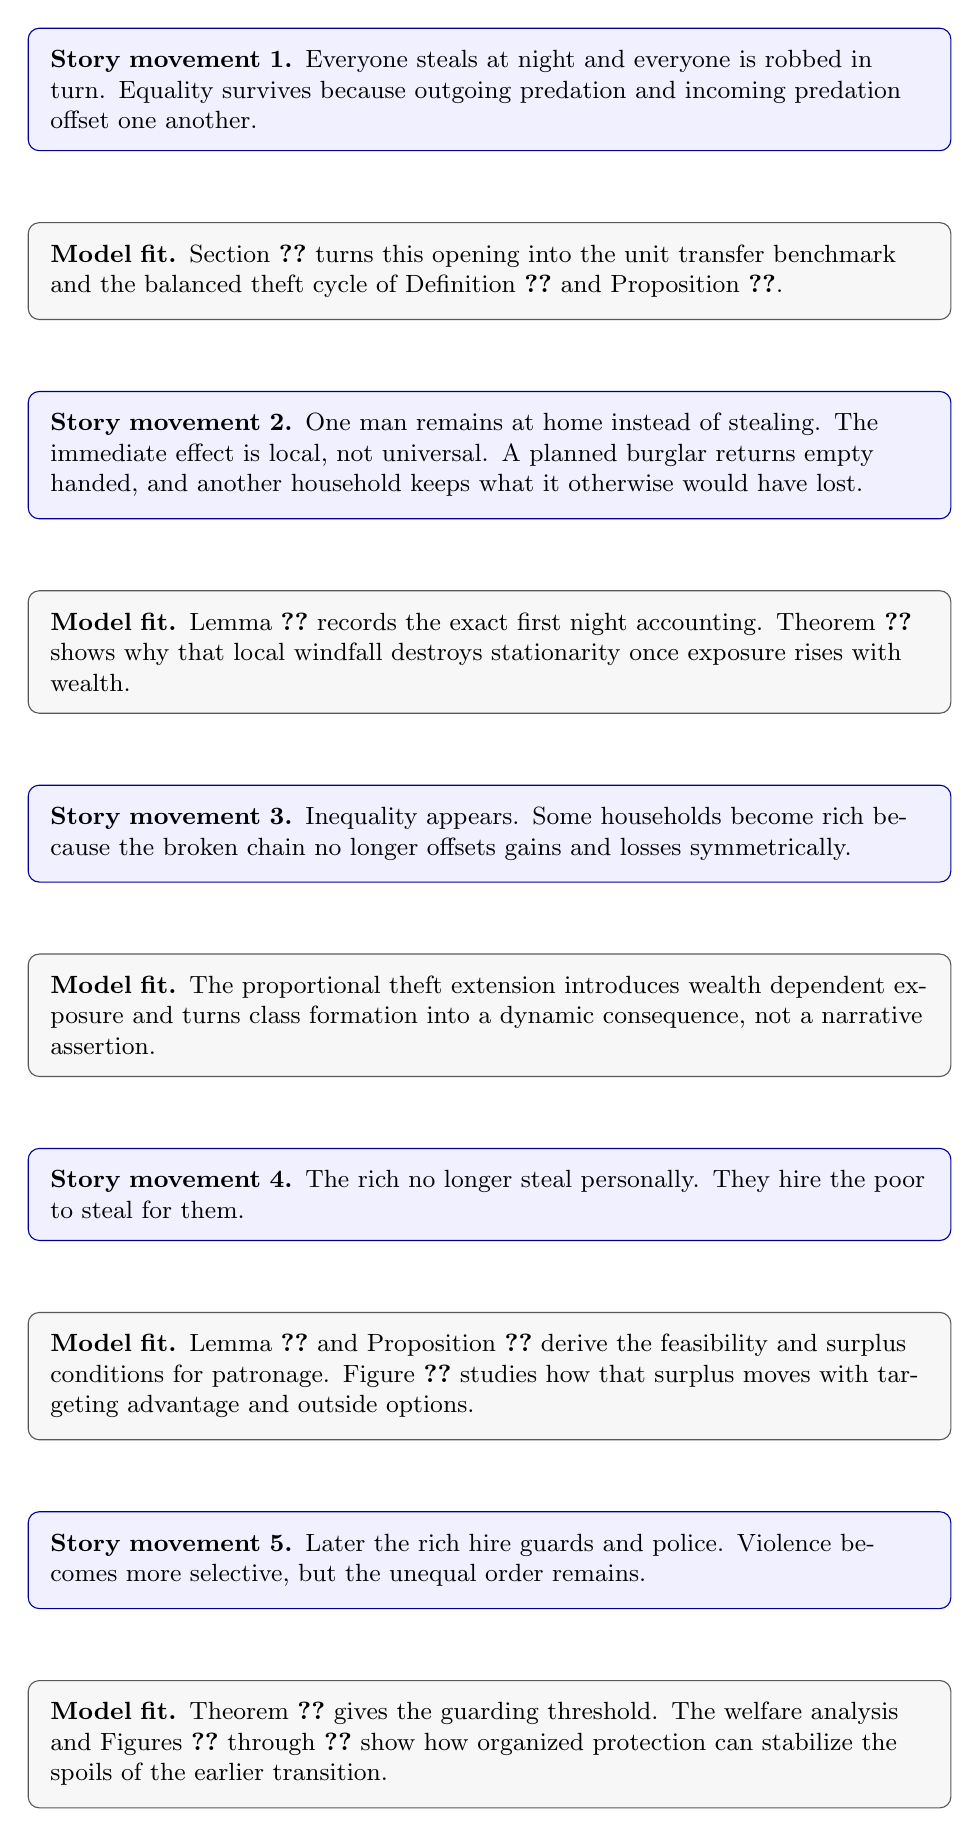
\begin{tikzpicture}[
        node distance = 0.9cm,
        every node/.style = {align=left, font=\small},
        story/.style = {draw=blue!60!black, rounded corners, fill=blue!6, text width=0.92\textwidth, inner sep=8pt},
        model/.style = {draw=black!65, rounded corners, fill=black!3, text width=0.92\textwidth, inner sep=8pt}
    ]
        \node[story] (s1) {\textbf{Story movement 1.} Everyone steals at night and everyone is robbed in turn. Equality survives because outgoing predation and incoming predation offset one another.};
        \node[model, below=of s1] (m1) {\textbf{Model fit.} Section \ref{sec:model} turns this opening into the unit transfer benchmark and the balanced theft cycle of Definition \ref{def:balanced-cycle} and Proposition \ref{prop:balanced-cycle}.};

        \node[story, below=of m1] (s2) {\textbf{Story movement 2.} One man remains at home instead of stealing. The immediate effect is local, not universal. A planned burglar returns empty handed, and another household keeps what it otherwise would have lost.};
        \node[model, below=of s2] (m2) {\textbf{Model fit.} Lemma \ref{lem:first-night} records the exact first night accounting. Theorem \ref{thm:no-stationary-one-honest} shows why that local windfall destroys stationarity once exposure rises with wealth.};

        \node[story, below=of m2] (s3) {\textbf{Story movement 3.} Inequality appears. Some households become rich because the broken chain no longer offsets gains and losses symmetrically.};
        \node[model, below=of s3] (m3) {\textbf{Model fit.} The proportional theft extension introduces wealth dependent exposure and turns class formation into a dynamic consequence, not a narrative assertion.};

        \node[story, below=of m3] (s4) {\textbf{Story movement 4.} The rich no longer steal personally. They hire the poor to steal for them.};
        \node[model, below=of s4] (m4) {\textbf{Model fit.} Lemma \ref{lem:contract-feasibility} and Proposition \ref{prop:patronage} derive the feasibility and surplus conditions for patronage. Figure \ref{fig:fig06_contracting_comparative_statics} studies how that surplus moves with targeting advantage and outside options.};

        \node[story, below=of m4] (s5) {\textbf{Story movement 5.} Later the rich hire guards and police. Violence becomes more selective, but the unequal order remains.};
        \node[model, below=of s5] (m5) {\textbf{Model fit.} Theorem \ref{thm:guarding} gives the guarding threshold. The welfare analysis and Figures \ref{fig:fig07_regime_phase_diagram} through \ref{fig:fig11_welfare_decomposition} show how organized protection can stabilize the spoils of the earlier transition.};
    \end{tikzpicture}
    \caption{Annotated passage map of the story by Calvino. The figure paraphrases the key narrative movements and indicates the point in the paper where each movement is formalized or simulated.}
    \label{fig:calvino-map}
\end{figure}


\end{document}
